\chapter{Reductions \texorpdfstring{$\bmod\ p$}{mod p} of the Basic Moduli Problems}
\label{ch:13}

\section{Some general considerations on crossings at supersingular points}
\label{sec:13.1}

\kmitem\label{item:13.1.1}
Let $k$ be a field. We suppose given
\[
\begin{tikzcd}[row sep=1.8em]
X \arrow[d] \\
Y \arrow[d] \\
\Spec(k)
\end{tikzcd}
\]
where
\begin{enumerate}[label=(\arabic*)]
\item $Y$ is a smooth curve over $k$
\item $X$ is finite and flat over $Y$.
\end{enumerate}
We further suppose given a non-empty finite set of $k$-valued points of $Y$, which we call the ``supersingular points,'' and we suppose that
\begin{enumerate}[label=(\arabic*), start=3]
\item Lying over each supersingular point $y_0$ of $Y$, there is a unique closed point $x_0$ of $X$, that point is $k$-rational, and the complete local ring of $X$ at $x_0$ is isomorphic to
\[
k[[x, y]]/(\text{one equation}) .
\]
\end{enumerate}
We further suppose given a finite collection of $k$-schemes $\{Z_i\}_{i \in I}$ which sit in a diagram
\[
\begin{tikzcd}[row sep=1.8em, column sep=large]
X \arrow[d] & \coprod_{i \in I} Z_i \arrow[l] \arrow[ld] \\
Y \arrow[d] & \\
\Spec(k) . &
\end{tikzcd}
\]
We assume that
\begin{enumerate}[label=(\arabic*), start=4]
\item For each $i \in I$, and each supersingular point $y_0$ of $Y$, there is a unique closed point $z_{i,0}$ of $Z_i$ lying over $y_0$, and this point $z_{i,0}$ is $k$-rational;
\item each $Z_i$ is finite and flat over $Y$;
\item each $(Z_i)^{\mathrm{red}}$ is a smooth curve over $k$;
\item for each $i$, $Z_i \to X$ is a closed immersion;
\item over the open set $Y - \{\text{s.s.\ points}\}$ of $Y$, the morphism
\[
\coprod_{i \in I} Z_i \to X
\]
is an isomorphism.
\end{enumerate}

\stepcounter{kmitem}
\begin{crossingsthm}\label{thm:13.1.3}
In the above situation, let $y_0$ be a supersingular point of $Y$, $x_0$ the unique closed point of $X$ lying over it. Then the complete local ring of $X$ at $x_0$ is of the form
\[
k[[x, y]] \Big/ \prod_{i \in I} f_i^{e_i} ,
\]
where the $f_i$'s are distinct-modulo-units irreducibles in the ring $k[[x, y]]$, and where, for each $i \in I$, the complete local ring
\[
k[[x, y]]/(f_i^{e_i})
\]
is isomorphic to the complete local ring of $Z_i$ at $z_{i,0}$.

If $Y$ is connected (respectively, geometrically connected), then so are the $Z_i$, and then the $Z_i$ are the irreducible components of $X$.
\end{crossingsthm}

\begin{proof}
Because $Y$ is smooth over $k$, and $y_0$ is $k$-rational, the complete local ring of $Y$ at $y_0$ is of the form $k[[T]]$. By hypothesis, the complete local ring of $X$ at $x_0$ is of the form
\[
k[[x, y]]/(\text{one equation}) .
\]
Because $X \to Y$ is finite flat, the ring extension
\[
\begin{tikzcd}[row sep=1.8em]
k[[x, y]]/(\text{one equation}) \\
k[[T]] \arrow[u]
\end{tikzcd}
\]
is finite flat. Therefore ``one equation'' is neither zero nor a unit in $k[[x, y]]$. Factoring it up-to-units into powers of distinct-up-to-units irreducibles in $k[[x, y]]$, the situation looks like
\[
\begin{tikzcd}[row sep=1.8em]
k[[x, y]]/\bigl(\prod_{j \in J} f_j^{e_j}\bigr) \\
k[[T]] , \arrow[u]
\end{tikzcd}
\]
where the $f_j$'s are indexed by some finite non-void indexing set $J$.

Now we exploit the fact that
\[
\begin{tikzcd}[row sep=1.8em]
k[[x, y]]/\bigl(\prod_{j \in J} f_j^{e_j}\bigr) \\
k[[T]] \arrow[u]
\end{tikzcd}
\]
is finite and flat of some degree $d \ge 1$. Let $T_1 \in k[[x, y]]$ be any element which reduces $\bmod \prod f_j^{e_j}$ to $T$. Then the quotient
\[
k[[x, y]]/\bigl(\prod f_j^{e_j}, T_1\bigr)
\]
is a $d$-dimensional $k$-vector space. Therefore $T_1$ is a non-unit, and it is non-zero. Let us write its factorization in $k[[x, y]]$ as
\[
T_1 = \prod g_k^{n_k} .
\]
Then for each pair $(j, k)$, the ring
\[
k[[x, y]]/(f_j, g_k)
\]
is a quotient of a finite-dimensional $k$-algebra, so is itself finite dimensional. Therefore we conclude that for all $(j, k)$, $f_j$ and $g_k$ are distinct-up-to-units irreducibles of $k[[x, y]]$.

Now consider the ring
\[
k[[x, y]][1/T_1] .
\]
It is a regular one-dimensional ring with unique factorization, and its irreducibles up-to-units are exactly
\[
\{\text{all irreducibles of } k[[x, y]]\} - \{\text{the irreducibles which divide } T_1\} .
\]
Therefore the $f_i$'s remain irreducible non-units in the ring
\[
k[[x, y]][1/T_1] .
\]
By the Chinese Remainder Theorem, we have
\[
k[[x, y]][1/T_1]\Big/\prod f_j^{e_j} \xrightarrow{\ \sim\ } \prod \bigl(k[[x, y]][1/T_1]/(f_j^{e_j})\bigr) ,
\]
and each factor
\[
k[[x, y]][1/T_1]/(f_j^{e_j})
\]
is itself an artin local ring. Thus we have a cartesian diagram
\[
\begin{tikzcd}[row sep=2em, column sep=small]
X \arrow[d] &
\begin{gathered}
\Spec\Bigl( \bigl(k[[x, y]]/\prod f_j^{e_j}\bigr) \\
\qquad\qquad\quad \tens{k[[T]]} k((T)) \Bigr)
\end{gathered}
  \arrow[l, hook'] \arrow[d] \arrow[r, "\sim"] &
\begin{gathered}
\coprod \Spec\Bigl( \bigl(k[[x, y]]/(f_j^{e_j})\bigr) \\
\qquad\qquad\qquad \tens{k[[T]]} k((T)) \Bigr)
\end{gathered}
  \arrow[ld] \\
Y & \Spec(k((T))) \arrow[l] &
\end{tikzcd}
\]
By hypothesis, over the open set $Y - \{\text{s.s.\ points}\}$, we have
\[
X \xleftarrow{\ \sim\ } \coprod Z_i ,
\]
so in particular over $\Spec(k((T))) \to Y - \{\text{s.s.\ points}\}$, we have
\[
X \fib{Y} \Spec(k((T))) \xleftarrow{\ \sim\ } \coprod_{i \in I} Z_i \fib{Y} \Spec(k((T))) .
\]
By assumption, $Z_i$ has a unique closed point $z_{i,0}$ lying over $x_0$, this point is $k$-rational, and $Z_i^{\mathrm{red}}$ is a smooth curve. Therefore
\[
Z_i \fib{Y} \Spec(k((T))) = \Spec\bigl( \widehat{\mathcal{O}}_{Z_i, z_{i,0}} \tens{k[[T]]} k((T)) \bigr) .
\]
This scheme is irreducible, because
\[
Z_i^{\mathrm{red}} \fib{Y} \Spec(k((T))) = \bigl( Z_i \fib{Y} \Spec(k((T))) \bigr)^{\mathrm{red}}
\]
is itself reduced and irreducible (being isomorphic to $k((z))$ for $z$ a uniformizing parameter at $z_{i,0}$ on $(Z_i)^{\mathrm{red}}$). Therefore we have an equality of $k((T))$-schemes
\[
\coprod_j \Spec\Bigl( \bigl(k[[x, y]]/(f_j^{e_j})\bigr) \tens{k[[T]]} k((T)) \Bigr) \simeq \coprod_i Z_i \fib{Y} \Spec(k((T))) ,
\]
each expressed as a disjoint union of irreducible schemes. Therefore there is a bijection of the two indexing sets, under which, for each $i$, we have an isomorphism of $k((T))$-algebras
\[
\bigl( k[[x, y]]/(f_i^{e_i}) \bigr) \tens{k[[T]]} k((T)) \simeq \widehat{\mathcal{O}}_{Z_i, z_{i,0}} \tens{k[[T]]} k((T)) .
\]
It remains to prove the final assertion. We must explain why the above isomorphism extends to an isomorphism
\[
\Spec(\widehat{\mathcal{O}}_{Z_i, z_{i,0}}) \xrightarrow{\ \sim\ } \Spec\bigl( k[[x, y]]/(f_i^{e_i}) \bigr) .
\]
Recall that we were given a diagram
\[
\begin{tikzcd}[row sep=1.8em, column sep=large]
X & Z_i \arrow[l] \arrow[ld] \\
Y &
\end{tikzcd}
\]
so we certainly have a homomorphism of complete local $k[[T]]$-algebras
\[
k[[x, y]]\Big/\prod_j f_j^{e_j} \to \widehat{\mathcal{O}}_{Z_i, z_{i,0}} .
\]
We first claim this map factors through the projection onto $k[[x, y]]/(f_i^{e_i})$. Consider the diagram
\[
\begin{tikzcd}[row sep=1.6em, column sep=small]
0 \arrow[r] & \Ker \arrow[r] \arrow[rd, "?"] \arrow[rdd, dashed] &
k[[x, y]]/\prod_j f_j^{e_j} \arrow[r] \arrow[d] & k[[x, y]]/(f_i^{e_i}) \arrow[r] & 0 \\
&& \widehat{\mathcal{O}}_{Z_i, z_{i,0}} \arrow[d, hook] && \\
&& \widehat{\mathcal{O}}_{Z_i, z_{i,0}} \tens{k[[T]]} k((T)) . &&
\end{tikzcd}
\]
The lowest vertical arrow is injective because $\widehat{\mathcal{O}}$ is flat over $k[[T]]$. We know that the dotted arrow vanishes, so we conclude that the diagonal arrow ``$?$'' also vanishes. This gives us a homomorphism
\[
k[[x, y]]/(f_i^{e_i}) \to \widehat{\mathcal{O}}_{Z_i, z_{i,0}} .
\]
We next remark that the $k[[T]]$-algebra
\[
k[[x, y]]/(f_i^{e_i})
\]
is flat over $k[[T]]$ (simply because it is finite over this regular ring of dimension one, and is itself Cohen-Macaulay of dimension one, being defined by one equation in a regular scheme of dimension two). Thus we have a homomorphism between \emph{free} $k[[T]]$-algebras of finite rank, which is an isomorphism after inverting $T$. Therefore it is \emph{injective}. It is surjective because it sits in
\[
k[[x, y]]\Big/\Bigl(\prod_j f_j^{e_j}\Bigr) \twoheadrightarrow k[[x, y]]/(f_i^{e_i}) \to \widehat{\mathcal{O}}_{Z_i, z_{i,0}} ,
\]
in which the composite is surjective because $Z_i \to X$ is a closed immersion.

It remains to show that each $Z_i$ is connected (resp.~geometrically connected) if $Y$ is. This is clear from the fact that $Z_i$ has a \emph{unique} point lying over each supersingular point of $Y$, and that $Z_i \to Y$ is finite and flat (compare \ref{cor:12.6.2}). Once $Z_i$ is connected, it is irreducible, because $(Z_i)^{\mathrm{red}}$ is a smooth curve over $k$.
\end{proof}

\begin{krem}\label{rem:13.1.4}
If all the $Z_i$ are reduced, then the crossings theorem shows that $X$ itself is reduced.
\end{krem}

\kmitem\label{item:13.1.5}\emph{Terminology.}\par
In the above situation, we will say that $X$ is ``the'' disjoint union of the $Z_i$'s with crossings at the supersingular points.

\kmitem\label{item:13.1.6}\emph{``Picture''} of three $Z_i$'s, three supersingular points, to be visualized as intersecting strings in 3-space.
\begin{center}
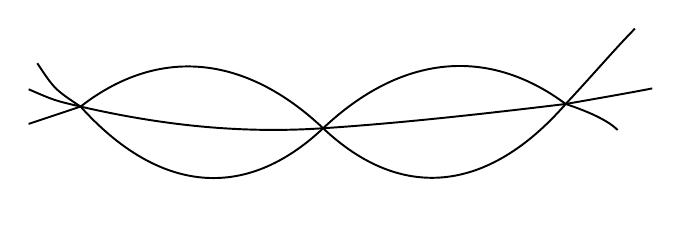
\begin{tikzpicture}[scale=1.1, line width=0.7pt]
  % Define the three crossing points
  \coordinate (P1) at (-2.8, 0.25);
  \coordinate (P2) at (0, 0);
  \coordinate (P3) at (2.8, 0.28);

  % Middle string (flatter, gently curving)
  \draw (-3.4, 0.45) .. controls (-3.1, 0.32) .. (P1)
        .. controls (-1.8, 0.02) and (-0.9, -0.06) .. (P2)
        .. controls (0.9, 0.06) and (1.8, 0.16) .. (P3)
        .. controls (3.2, 0.35) and (3.6, 0.42) .. (3.8, 0.46);

  % String 1 (starts low, loops high between P1 and P2, loops low between P2 and P3, ends high)
  \draw (-3.4, 0.05) .. controls (-3.1, 0.15) .. (P1)
        .. controls (-1.9, 0.95) and (-0.9, 0.85) .. (P2)
        .. controls (0.9, -0.85) and (1.9, -0.75) .. (P3)
        .. controls (3.1, 0.6) and (3.4, 0.95) .. (3.6, 1.15);

  % String 2 (starts high, loops low between P1 and P2, loops high between P2 and P3, ends low)
  \draw (-3.3, 0.75) .. controls (-3.1, 0.45) .. (P1)
        .. controls (-1.9, -0.75) and (-0.9, -0.85) .. (P2)
        .. controls (0.9, 0.85) and (1.9, 0.95) .. (P3)
        .. controls (3.1, 0.18) and (3.3, 0.08) .. (3.4, -0.02);
\end{tikzpicture}
\end{center}

\kmitem\label{item:13.1.7}\emph{More terminology}\par
Suppose we are given a diagram
\[
\begin{tikzcd}[row sep=1.8em, column sep=large]
X \arrow[d] & \coprod Z_i \arrow[l] \arrow[ld] \\
Y \arrow[d] & \\
\Spec(k) &
\end{tikzcd}
\]
and a closed subscheme in $Y$, finite etale over $\Spec(k)$, of ``supersingular points.'' Suppose that axioms 1), 2), 5), 6), 7), 8) hold, and that axioms 3) and 4) become \emph{true} after extending scalars to a separable closure $\bar{k}$ of $k$. We will still say in this situation that $X$ is the disjoint union of the $Z_i$'s with crossings at the supersingular points.

\section{Modular schemes as examples}
\label{sec:13.2}

\kmitem\label{item:13.2.1}
Let $\Gamma$ be a subgroup of $\GL(2, \mathbb{Z}/p^n\mathbb{Z})$, $A$ the ring $(\mathbb{Z}[\zeta_{p^n}])^{\det(\Gamma)} \subset \mathbb{Z}[\zeta_{p^n}]$. Consider the moduli problem
\[
([\Gamma(p^n)]/\Gamma)^{A\text{-\rm can}} \quad\text{on}\quad (\mathrm{Ell}/A) .
\]
Suppose that it is a regular moduli problem. By (\ref{cor:9.1.8}), this is equivalent to the regularity of the moduli problem $[\Gamma(p^n)]/\Gamma$ on $(\mathrm{Ell}/\mathbb{Z})$, and we have seen (\ref{thm:7.6.1}) that this problem is regular for each of the following $\Gamma$'s:
\[
\left\{
\begin{aligned}
&\text{any } \Gamma \text{ contained in the ``semi Borel'' } \begin{pmatrix} 1 & * \\ 0 & * \end{pmatrix} \\
&\Gamma = \begin{pmatrix} H_1 & 0 \\ 0 & H_2 \end{pmatrix} \quad\text{for } H_1, H_2 \text{ subgroups of } (\mathbb{Z}/p^n\mathbb{Z})^\times \\
&\Gamma = \begin{pmatrix} H_1 & * \\ 0 & H_2 \end{pmatrix} \quad\text{for } H_1, H_2 \text{ subgroups of } (\mathbb{Z}/p^n\mathbb{Z})^\times \\
&\qquad\qquad\qquad\quad\ \ \text{and } * \text{ unrestricted in } \mathbb{Z}/p^n\mathbb{Z} .
\end{aligned}
\right.
\]

\begin{kthm}\label{thm:13.2.2}
Let $k$ be a perfect field of characteristic $p$, $\mathcal{S}$ a representable moduli problem on $(\mathrm{Ell}/k)$ which is finite etale over $(\mathrm{Ell}/k)$, and such that all the supersingular points on $\mathfrak{M}(\mathcal{S})$ are $k$-rational.
\begin{enumerate}[label=\arabic*)]
\item Let $\Gamma \subset \GL(2, \mathbb{Z}/p^n\mathbb{Z})$ be a subgroup such that the moduli problem $([\Gamma(p^n)]/\Gamma)^{A\text{-\rm can}}$ is regular, and denote by
\[
\mathcal{P} = ([\Gamma(p^n)]/\Gamma)^{A\text{-\rm can}} \tens{A} k
\]
the moduli problem on $(\mathrm{Ell}/k)$ deduced by the unique ring homomorphism $A \to k$. Then the moduli spaces
\[
\begin{tikzcd}[row sep=1.8em]
X = \mathfrak{M}(\mathcal{S}, \mathcal{P}) \arrow[d] \\
Y = \mathfrak{M}(\mathcal{S}) \arrow[d] \\
\Spec(k)
\end{tikzcd}
\]
satisfy 1), 2), 3) of the Crossings Theorem (\ref{thm:13.1.3}).
\item For any $n \ge 1$, the moduli spaces
\[
\begin{tikzcd}[row sep=1.8em]
X = \mathfrak{M}(\mathcal{S}, [p^n\text{-\rm Isog}]) \arrow[d] \\
Y = \mathfrak{M}(\mathcal{S}) \arrow[d] \\
\Spec(k)
\end{tikzcd}
\]
satisfy hypotheses 1), 2), 3) of the Crossings theorem.
\end{enumerate}
\end{kthm}

\begin{proof}
Because $\mathcal{S}$ is finite etale over $(\mathrm{Ell}/k)$, $\mathfrak{M}(\mathcal{S})$ is a smooth curve over $k$. The regular moduli problems (resp.~$[p^n\text{-\rm Isog}]$) are finite flat over $(\mathrm{Ell}/A)$ (resp.~over $(\mathrm{Ell}/\mathbb{Z})$); in the first case because a finite map between regular two-dimensional schemes is flat, in the second because we have proven it (\ref{thm:6.8.1}). Let $y_0$ be a $k$-valued point of $Y = \mathfrak{M}(\mathcal{S})$ which is supersingular, corresponding to a supersingular elliptic curve $E_0/k$ together with an element $a \in \mathcal{S}(E_0/k)$. Then a closed point of $X = \mathfrak{M}(\mathcal{S}, \mathcal{P})$ lying over $y_0$ is the image of a closed point in $\mathfrak{M}(\mathcal{S}, [\Gamma(p^n)])$ lying over $y_0$. But there is a unique closed point of $\mathfrak{M}(\mathcal{S}, [\Gamma(p^n)])$ lying over $y_0$, and it is $k$-rational. To see this recall that such a closed point ``is'' a Drinfeld $p^n$-basis of $E_0 \tens{k} k'/k'$ for some finite extension field $k'/k$; as $E_0$ is supersingular we have $E_0[p^n](k') = 0$, so $(0, 0)$ is the unique possible Drinfeld $p^n$-basis, and it is $k$-rational. For $X = \mathfrak{M}(\mathcal{S}, [p^n\text{-\rm Isog}])$ the argument is similar; the unique closed point lying over $y_0$ is the unique subgroup of $E_0 \tens{k} \bar{k}$ of rank $p^n$, namely $\Ker(F_0^n)$, and it is $k$-rational.

It remains to explain why the complete local ring at the unique point $x_0$ of $X$ lying over $y_0$ is of the form
\[
k[[x, y]]/(\text{one equation}) .
\]
In the case of $\mathfrak{M}(\mathcal{S}, [p^n\text{-\rm Isog}])$, the argument given in (\ref{thm:6.8.2}), applied to the deformation theory of $p^n$-isogenies over artin local $k$-algebras with residue field $k$, shows that the complete local ring of $\mathfrak{M}(\mathcal{S}, [p^n\text{-\rm Isog}])$ at any $k$-valued supersingular point is of the form
\[
k[[x, y]]/(\text{one equation}) ,
\]
where $x$ and $y$ are the local ``$T$-coordinates'' for the source and target of the isogeny.

In the case of $\mathfrak{M}(\mathcal{S}, \mathcal{P})$, we argue as follows. The spectrum of the complete local ring of $\mathfrak{M}(\mathcal{S}, \mathcal{P})$ at a $k$-valued supersingular point lying over $y_0 = (E_0/k, a)$ is (tautologically) equal to
\[
\mathcal{P}_{E_0/k[[T]]} ,
\]
where $E_0/k[[T]]$ denotes the universal deformation of $E_0$ to a complete local $k$-algebra with residue field $k$. Let $E/W(k)[[T]]$ denote the universal deformation of $E_0$ to a complete local ring with residue field $k$. Then $E \tens{\mathbb{Z}} A / (A \tens{\mathbb{Z}} W(k))[[T]]$ is the universal formal deformation of $E_0$ to a complete local $A$-algebra with residue field $k$ (for $A = (\mathbb{Z}[\zeta_{p^n}])^{\det(\Gamma)}$, $A \tens{\mathbb{Z}} W(k)$ is a complete discrete valuation ring with residue field $k$!).

By definition
\begin{align*}
\mathcal{P}_{E_0/k[[T]]} &= k \tens{A} \bigl( ([\Gamma(p^n)]/\Gamma)^{A\text{-\rm can}} \bigr)_{\substack{\textstyle E \tens{\mathbb{Z}} A / \\ \textstyle (A \tens{\mathbb{Z}} W(k))[[T]]}} \\
&= k \tens{A} \bigl( ([\Gamma(p^n)]/\Gamma) \bigr)_{E / W(k)[[T]]} \\
&= k \tens{A} \begin{pmatrix}
\text{the spectrum of a two-dimensional} \\
\text{complete regular local } A\text{-algebra} \\
\text{with residue field } k
\end{pmatrix} \\
&= k \tens{A \tens{\mathbb{Z}} W(k)} \begin{pmatrix}
\text{the spectrum of a two-dimensional} \\
\text{complete regular local} \\
A \tens{\mathbb{Z}} W(k)\text{-algebra} \\
\text{with residue field } k .
\end{pmatrix} .
\end{align*}
Again because $A \tens{\mathbb{Z}} W(k)$ is a complete discrete valuation ring with residue field $k$, any two-dimensional complete regular local $A \tens{\mathbb{Z}} W(k)$-algebra with residue field $k$ is of the form
\[
(A \tens{\mathbb{Z}} W(k))[[x, y]]/(f)
\]
for some $f$ lying in $\mathfrak{m}$ but not in $\mathfrak{m}^2$. Tensoring over $A \tens{\mathbb{Z}} W(k)$ with $k$, we obtain
\[
\mathcal{P}_{E_0/k[[T]]} \simeq \text{the } \Spec \text{ of } k[[x, y]]/(\text{one equation}) . \qedhere
\]
\end{proof}

\section{Analysis of \texorpdfstring{$p$}{p}-power isogenies between elliptic curves}
\label{sec:13.3}

\begin{kprop}\label{prop:13.3.1}
Let $E/S/\mathbb{F}_p$ be an ordinary elliptic curve over an $\mathbb{F}_p$-scheme. For every integer $n \ge 1$, the ``standard factorization'' of the cyclic $p^{2n}$-isogeny ``multiplication by $p^n$'' into two cyclic $p^n$-isogenies is
\[
E \xrightarrow{\ F^n\ } E^{(p^n)} \xrightarrow{\ V^n\ } E .
\]
The kernel of $V^n$ is a finite etale $S$-group, locally (etale) on $S$ isomorphic to $\mathbb{Z}/p^n\mathbb{Z}$, and the kernel of $F^n$ is its Cartier dual, locally (etale) on $S$ isomorphic to $\mu_{p^n}$.
\end{kprop}

\begin{proof}
The first assertion is (\ref{lem:12.2.5}). The finite etale $S$-scheme which makes the second true is none other than
\[
[\mathrm{Ig}(p^n)]_{E/S} . \qedhere
\]
\end{proof}

\begin{kprop}\label{prop:13.3.2}
Let $E/S/\mathbb{F}_p$ be an ordinary elliptic curve over an $\mathbb{F}_p$-scheme, $n \ge 1$ an integer, and $G \subset E$ a finite locally free $S$-subgroup-scheme of rank $p^n$. Then Zariski locally on $S$ there exists a unique pair of integers $a, b$ with $a \ge 0$, $b \ge 0$, $a + b = n$, such that
\begin{enumerate}[label=\arabic*)]
\item $G \cap \Ker F^n = \Ker F^a$ is a twisted $\mu_{p^a}$;
\item $G \bmod \Ker F^a$ is finite etale cyclic of order $p^{n-a}$.
\end{enumerate}
\end{kprop}

\begin{proof}
The group $E[p^n]$ sits in the short exact sequence
\[
0 \to \Ker F^n \to E[p^n] \xrightarrow{\ F^n\ } \Ker V^n \to 0
\]
with $\Ker V^n$ a twisted $\mathbb{Z}/p^n\mathbb{Z}$. Consider the composite map
\[
\begin{tikzcd}[row sep=1.8em, column sep=large]
G \arrow[d, hook] \arrow[rd, dashed] & \\
E[p^n] \arrow[r, "F^n"'] & \Ker V^n .
\end{tikzcd}
\]
By (\ref{cor:4.10.1}), this dotted arrow maps $G$ onto a finite etale subgroup $H'$ of $\Ker V^n$, which Zariski locally on $S$ can be none other than the twisted $\mathbb{Z}/p^b\mathbb{Z}$ which is $\Ker(V^b : E^{(p^n)} \to E^{(p^{n-b})})$. Therefore the kernel of the dotted arrow is a finite locally free subgroup of $G$. The kernel of the dotted arrow is $G \cap \Ker F^n$, and therefore $G \cap \Ker(F^n)$ is a finite locally free subgroup of $\Ker(F^n)$. Because $\Ker(F^n)$ is a twisted $\mu_{p^n}$, $G \cap \Ker(F^n)$ can be none other than one of the subgroups $\Ker(F^a : E \to E^{(p^a)})$. Comparing ranks, we see that $a + b = n$.
\end{proof}

\begin{kthm}\label{thm:13.3.3}
Let $E_0, E_n$ be ordinary elliptic curves over a connected $\mathbb{F}_p$-scheme $S$, and let
\[
E_0 \xrightarrow{\ \pi_{0,n}\ } E_n
\]
be a $p^n$-isogeny, $n \ge 1$. Then there exist unique integers $a, b \ge 0$, $a + b = n$, such that this isogeny factors as
\[
E_0 \xrightarrow{\ F_0^a\ } E_0^{(p^a)} \xrightarrow[\varepsilon]{\ \sim\ } E_n^{(p^b)} \xrightarrow{\ V_n^b\ } E_n ,
\]
where $F_0$ denotes the Frobenius for $E_0$, $V_n$ denotes the Verschiebung for $E_n$, and where $\varepsilon$ is an isomorphism of elliptic curves over $S$.
\end{kthm}

\begin{proof}
By the previous proposition, applied to $G = \Ker(\pi_{0,n})$, we have a short exact sequence
\[
0 \to \Ker(F^a) \to G \to \text{a twisted } \mathbb{Z}/p^b\mathbb{Z} \to 0 .
\]
Therefore our isogeny factors as
\[
E_0 \xrightarrow{\ F_0^a\ } E_0^{(p^a)} \xrightarrow{\ \pi_{a,n}\ } E_n
\]
where $\pi_{a,n}$ is a $p^b$-isogeny whose kernel is a twisted $\mathbb{Z}/p^b\mathbb{Z}$. Therefore its dual
\[
E_0^{(p^a)} \xleftarrow{\ \pi^t_{a,n}\ } E_n
\]
has kernel a twisted $\mu_{p^b}$. Applying (\ref{prop:13.3.2}) to $\Ker(\pi^t_{a,n})$, we see that we must have $\Ker(\pi^t_{a,n}) = \Ker(F^b_n : E_n \to E_n^{(p^b)})$.
\end{proof}

\kmitem\label{item:13.3.4}
We will call an isogeny of the form
\[
E_0 \xrightarrow{\ F_0^a\ } E_0^{(p^a)} \xrightarrow[\varepsilon]{\ \sim\ } E_n^{(p^b)} \xrightarrow{\ V_n^b\ } E_n
\]
a $p^n$-isogeny of type $(a, b)$, or an $(a,b)$ isogeny if $p$ is understood. We next will analyze when an $(a,b)$ isogeny between \emph{ordinary} elliptic curves is cyclic. For this it is convenient to introduce an auxiliary rigidification.

\begin{kthm}\label{thm:13.3.5}
Let $k$ be a perfect field of characteristic $p$, and $\mathcal{P}$ a representable moduli problem on $(\mathrm{Ell}/k)$ which is finite etale over $(\mathrm{Ell}/k)$. Consider an $(a,b)$ isogeny between elliptic curves over a $k$-scheme $S$ :
\[
E_0 \xrightarrow{\ F_0^a\ } E_0^{(p^a)} \xrightarrow[\varepsilon]{\ \sim\ } E_n^{(p^b)} \xrightarrow{\ V_n^b\ } E_n .
\]
Let $a_0 \in \mathcal{P}(E_0/S)$ be a level $\mathcal{P}$-structure on $E_0/S$. Denote by
\[
a_a \xlongequal{\mathrm{dfn}} (a_0)^{(p^a)} \in \mathcal{P}^{(\sigma^a)}(E_0^{(p^a)}/S) ,
\]
\[
\beta_n \in \mathcal{P}^{(\sigma^{a-b})}(E_n/S) \text{ the unique element such that}
\]
\[
\text{in } \mathcal{P}^{(\sigma^a)}(E_n^{(p^b)}/S), \text{ we have } (\beta_n)^{(p^b)} = (\varepsilon^{-1})^*(a_a) .
\]
Denote by
\[
x_0 \in \mathfrak{M}(\mathcal{P})(S) \text{ the isomorphism class of } (E_0/S, a_0) ,
\]
\[
x_n \in \mathfrak{M}(\mathcal{P}^{(\sigma^{a-b})})(S) \text{ the isomorphism class of } (E_n/S, \beta_n) ,
\]
and by $F : \mathfrak{M}(\mathcal{P}^{(\sigma^i)}) \to \mathfrak{M}(\mathcal{P}^{(\sigma^{i+1})})$ the relative-to-$k$ Frobenius. Then we have the following results:
\begin{enumerate}[label=(\arabic*)]
\item $F^a(x_0) = F^b(x_n)$ in $\mathfrak{M}(\mathcal{P}^{(\sigma^a)})(S)$.
\item If $a = 0$ or if $b = 0$, then any $(a,b)$ isogeny is cyclic.
\item If both $a \ge 1$ and $b \ge 1$, and if the point
\[
(F^{a-1}(x_0), F^{b-1}(x_n)) \in \bigl( \mathfrak{M}(\mathcal{P}^{(\sigma^{a-1})}) \fib{k} \mathfrak{M}(\mathcal{P}^{(\sigma^{a-1})}) \bigr)(S)
\]
lies in the $p-1$'st infinitesimal neighborhood of the diagonal (i.e., the closed subscheme defined by the $p-1$'st power of the diagonal ideal), then the $(a,b)$ isogeny in question is cyclic.
\item If both $a \ge 1$ and $b \ge 1$, and if $E_0/S$ is ordinary, then the necessary and sufficient condition that the $(a,b)$ isogeny in question be cyclic is that the point $(F^{a-1}(x_0), F^{b-1}(x_n))$ lie in the $p-1$'st infinitesimal neighborhood of the diagonal.
\item If both $a \ge 1$ and $b \ge 1$, and if $E_0/S$ is ordinary with $j(E_0)(j(E_0)-1728)$ invertible on $S$, then the $(a,b)$ isogeny in question is cyclic if and only if the $j$-invariants of $E_0$ and $E_n$ satisfy the equation
\[
\bigl( j(E_0)^{p^{a-1}} - j(E_n)^{p^{b-1}} \bigr)^{p-1} = 0 .
\]
\end{enumerate}
\end{kthm}

\begin{proof}
Assertion (1) is obvious, for by construction $F^a(x_0)$ is the isomorphism class of $(E_0^{(p^a)}, a_a)$, $F^b(x_n)$ is the isomorphism class of $(E_n^{(p^b)}, (\varepsilon^{-1})^*(a_a))$, and $\varepsilon$ is an $S$-isomorphism between them. Assertion (2) is just the fact that $F^n$ and $V^n$ are always cyclic isogenies (\ref{lem:12.2.1}, \ref{lem:12.2.3}). Assertions (3) and (5) both follow from the key assertion (4). Admitting (4) for the moment, let us deduce (3) and (5). To obtain (3), we may reduce to the universal case in which $S$ is the fibre-product
\[
\begin{tikzcd}[row sep=2em, column sep=large]
S \arrow[r] \arrow[d, hook] & \mathrm{Inf}^{p-1}(\Delta) \arrow[d, hook] \\
\mathfrak{M}(\mathcal{P}) \fib{k} \mathfrak{M}(\mathcal{P}^{(\sigma^{a-b})}) \arrow[r, "{(F^{a-1}, F^{b-1})}"] & \mathfrak{M}(\mathcal{P}^{(\sigma^{a-1})}) \fib{k} \mathfrak{M}(\mathcal{P}^{(\sigma^{a-1})}) .
\end{tikzcd}
\]
The $\mathfrak{M}(\mathcal{P}^{(\sigma^i)})$ are all smooth curves over $k$, so the bottom horizontal arrow is finite and flat (of degree $p^{a+b-2}$). Therefore $S$ is finite flat over $\mathrm{Inf}^{p-1}(\Delta)$. But $\mathrm{Inf}^{p-1}(\Delta)$ is, by either projection, finite flat over $\mathfrak{M}(\mathcal{P}^{(\sigma^{a-1})})$ of degree $p-1$. Therefore $S$ is finite flat over $\mathfrak{M}(\mathcal{P}^{(\sigma^{a-1})})$. Therefore the open set $S^{\mathrm{ord}}$ of $S$ over which $E_0$ is ordinary is schematically dense in $S$ (because it is the inverse image of the open set $\mathfrak{M}(\mathcal{P}^{(\sigma^{a-1})})^{\mathrm{ord}}$, which is the complement of a finite set of points in a smooth curve). By (4), our isogeny is cyclic over $S^{\mathrm{ord}}$. But the condition that an isogeny be cyclic is represented by a closed subscheme of the base $S$. This closed subscheme contains $S^{\mathrm{ord}}$, so it must be all of $S$.

To deduce (5) from (4), we just use the fact that the map
\[
\mathfrak{M}(\mathcal{P}^{(\sigma^{a-1})}) \xrightarrow{\ j\ } \Spec(k[j])
\]
is finite etale where $j(j-1728)$ is invertible, and the fact that by (1), the point $(F^{a-1}(x_0), F^{b-1}(x_n))$ certainly lies in $\mathrm{Inf}^p(\Delta)$. So if $j(j-1728)$ is invertible, we may test whether or not we actually lie in $\mathrm{Inf}^{p-1}(\Delta)$ by passing to $j$-invariants.

It remains to prove (4). The individual isogenies
\[
E_0 \xrightarrow{\ F_0^a\ } E_0^{(p^a)} , \quad E_0^{(p^a)} \xrightarrow[\varepsilon]{\ \sim\ } E_n^{(p^b)} \xrightarrow{\ V_n^b\ } E_n ,
\]
are certainly cyclic, and the second one is etale, because $E_0$, and hence $E_n$, are ordinary. Therefore by (\ref{prop:6.7.8}), their composition is cyclic if and only if it is cyclic in standard order. Therefore our isogeny is cyclic if and only if, when it is written as the standard factorization of $F_0^a$, followed by the standard factorization of $V_n^b$, it is cyclic in standard order:
\[
\begin{tikzcd}[row sep=1.4em, column sep=1.7em]
E_0 \arrow[r, "F_0"] & E_0^{(p)} \arrow[r, "F_0^{(p)}"] & E_0^{(p^2)} \arrow[r, "\cdots"] & E_0^{(p^{a-1})} \arrow[d, "F_0^{(p^{a-1})}"] \\
& & & E_0^{(p^a)} \arrow[d] \\
& & & E_n .
\end{tikzcd}
\]
By (\ref{thm:6.7.15}), such a composite is cyclic in standard order if and only if each two-step composite is cyclic in standard order. The two-step composites consisting of adjacent $F$'s or of adjacent $V$'s are certainly cyclic in standard order (\ref{lem:12.2.4}). So the only ``weak link'' in our chain is the vertically drawn
\[
E_0^{(p^{a-1})} \xrightarrow{\ F_0^{(p^{a-1})}\ } E_0^{(p^a)} \xrightarrow[\varepsilon]{\ \sim\ } E_n^{(p^b)} \xrightarrow{\ V_n^{(p^{b-1})}\ } E_n^{(p^{b-1})} .
\]

This reduces us to the case $a = b = 1$. We must show that if $E_0/S/k$ is ordinary, and we are given $a_0 \in \mathcal{P}(E_0/S)$, then
\[
E_0 \xrightarrow{\ F_0\ } E_0^{(p)} \xrightarrow[\varepsilon]{\ \sim\ } E_2^{(p)} \xrightarrow{\ V_2\ } E_2
\]
is cyclic in standard order if and only if $(x_0, x_2)$ lies in $\mathrm{Inf}^{p-1}(\Delta)$ inside $\mathfrak{M}(\mathcal{P})^{\mathrm{ord}} \fib{k} \mathfrak{M}(\mathcal{P})^{\mathrm{ord}}$. The universal case of a $(1,1)$ isogeny with $\mathcal{P}$-structure on the (ordinary) source lives over $\mathrm{Inf}^p(\Delta)$. We must show that inside this $\mathrm{Inf}^p(\Delta)$, the locus of cyclicity is exactly the closed subscheme $\mathrm{Inf}^{p-1}(\Delta)$. It is enough to test the equality of two closed subschemes of a $k$-scheme of finite type by comparing points with values in artin local $k$-algebras with algebraically closed residue fields.

Thus we are reduced to the case when $S$ is $\Spec(R)$, with $R$ an artin local $k$-algebra with algebraically closed residue field. Over the residue field, the points $x_0, x_2$ simply coincide. So we may identify the special fibers of $(E_0, a_0)$ and $(E_2, \beta_2)$ once and for all, to a fixed $(E_{00}, a_{00})$. Let us also fix an isomorphism of $p$-divisible groups
\[
E_{00}[p^\infty] \simeq \mu_{p^\infty} \times \mathbb{Q}_p/\mathbb{Z}_p .
\]
Then there exist principal units (cf.~\ref{sec:8.9})
\[
q_0, q_2 \in 1 + \max(R)
\]
such that the $p$-divisible groups of $E_0/R$ and of $E_2/R$ are given by
\[
E_0[p^\infty] \simeq \mathbf{T}[p^\infty] \tens{\mathbb{Z}[q, q^{-1}]} R \quad\text{by } q \mapsto q_0
\]
\[
E_2[p^\infty] \simeq \mathbf{T}[p^\infty] \tens{\mathbb{Z}[q, q^{-1}]} R \quad\text{by } q \mapsto q_2 .
\]
We are given
\[
(q_0)^p = (q_2)^p .
\]
We must prove that $(q_0 - q_2)^{p-1} = 1$ if and only if
\[
E_0 \xrightarrow{\ F_0\ } E_0^{(p)} = E_2^{(p)} \xrightarrow{\ V_2\ } E_2
\]
is cyclic in standard order.

To analyze this question, we write the $p$-divisible groups explicitly. For any $R$-algebra $B$, with connected spectrum, $E_0[p^\infty](B)$ is the $p$-primary torsion subgroup of
\[
(B^\times) \times (\mathbb{Z}[1/p]) \big/ \bigl( \text{the cyclic subgroup generated by } (q_0, 1) \bigr) ,
\]
and similarly for $E_2$, with $q_0$ replaced by $q_2$. The groups for $E_0^{(p)} \simeq E_2^{(p)}$ are formed with $q_0$ replaced by $(q_0)^p = (q_2)^p$.

The Frobenius
\[
F_0 : E_0[p^\infty](B) \to E_0^{(p)}[p^\infty](B)
\]
is given by
\[
(X, a/p^n) \xrightarrow{\ F_0\ } (X^p, a/p^n) .
\]
The Verschiebung
\[
V_2 : E_2^{(p)}[p^\infty](B) \to E_2[p^\infty](B)
\]
is given by
\[
(X, a/p^n) \xrightarrow{\ V_2\ } (X, pa/p^n) .
\]

We are now in a position to apply the standard order criterion (\ref{thm:6.7.13}). Over the finite flat $R$-algebra
\[
R' = R[Z]/(Z^p = q_2)
\]
the point
\[
P = (Z, 1/p) \in E_0[p](R')
\]
has
\[
F_0(P) = (q_2, 1/p) \in E_2^{(p)}[p](R') ,
\]
and this point is visibly a generator of $\Ker V_2$. Therefore our composite $V_2 \circ F_0$ is cyclic in standard order if and only if $pP$ generates $\Ker F_0$. But we readily calculate in $E_0[p](R')$
\[
p(P) = p(Z, 1/p) = (Z^p, 1) = (q_2, 1) = (q_2/q_0, 0)
\]
so our composite is cyclic in standard order if and only if $q_2/q_0$ generates $\Ker F_0 \simeq \mu_p$, i.e., if and only if $q_2/q_0$ is a \emph{primitive} $p$'th root of unity. In characteristic $p$,
\[
\Phi_p(X) = \frac{X^p - 1}{X - 1} = (X-1)^{p-1} ,
\]
so
\begin{align*}
\Phi_p(q_2/q_0) = 0 &\iff \bigl( (q_2/q_0) - 1 \bigr)^{p-1} = 0 \\
&\iff (q_2 - q_0)^{p-1} = 0 . \qedhere
\end{align*}
\end{proof}


\section[Global structure of the moduli spaces]{Global structure of the moduli spaces \texorpdfstring{$\mathfrak{M}(\mathcal{P}, [\Gamma_0(p^n)])$}{M(P,[Gamma_0(p^n)])}, \texorpdfstring{$\mathfrak{M}(\mathcal{P}, [p^n\text{-Isog}])$}{M(P,[p^n-Isog])}}
\label{sec:13.4}

\begin{definition}\label{def:13.4.1}
Let $E/S/\mathbb{F}_p$ be an elliptic curve over an $\mathbb{F}_p$-scheme. Let $a, b$ be two integers, both $\ge 0$, with $a + b = n \ge 1$. A finite locally free $S$-subgroup-scheme $G \subset E$ of rank $p^n$ is said to be an $(a,b)$-\emph{subgroup} if the following two conditions are satisfied:
\begin{enumerate}[label=(\arabic*)]
\item $\Ker F^a \subset G$
\item in the resulting factorization of the isogeny with kernel $G$ as
\[
E \xrightarrow{\ F^a\ } E^{(p^a)} \xrightarrow{\ \pi_{a,n}\ } E_n = E \bmod G ,
\]
we have $\Ker(\pi^t_{a,n}) = \Ker(F^b_n)$.
\end{enumerate}
\end{definition}

\kmitem\label{item:13.4.2}
Thus if $G$ is an $(a,b)$ subgroup, then there exists an $S$-isomorphism $E^{(p^a)} \simeq E_n^{(p^b)}$.

\kmitem\label{item:13.4.3}
We say that $G$ is an \emph{$(a,b)$-cyclic group} if both conditions 1), 2) above are satisfied, and either $a = 0$ or $b = 0$, or the following condition is satisfied:
\begin{enumerate}[label=(\arabic*), start=3]
\item the two elliptic curves $E^{(p^{a-1})}, E_n^{(p^{b-1})}$ over $S$, whose ``$p$'th powers'' $E^{(p^a)}$ and $E_n^{(p^b)}$, are $S$-isomorphic, are themselves ``infinitesimally near each other to order $p-1$'', in the sense that there exists a closed subscheme of $S$ defined by an ideal whose $p-1$'st power is zero, over which the given isomorphism between $E^{(p^a)}$ and $E_n^{(p^b)}$ is induced by an isomorphism between $E^{(p^{a-1})}$ and $E_n^{(p^{b-1})}$.
\end{enumerate}

\begin{kprop}\label{prop:13.4.4}
Let $k$ be a perfect field of characteristic $p$, $\mathcal{P}$ a representable moduli problem on $(\mathrm{Ell}/k)$ which is finite etale over $(\mathrm{Ell}/k)$. For any integers $a \ge 0$, $b \ge 0$ with $a + b = n \ge 1$, the moduli problem on $(\mathrm{Ell}/k)$ defined by
\[
\begin{aligned}
{}[\mathcal{P}, (a,b)](E/S) = \{ & a \in \mathcal{P}(E/S), \text{ plus an} \\
& (a,b)\text{-subgroup } G \text{ in } E/S \}
\end{aligned}
\]
is represented by the finite flat $\mathfrak{M}(\mathcal{P})$-scheme of degree $p^b$
\[
\mathfrak{M}(\mathcal{P}, (a,b)) = (F^a \times F^b)^{-1}(\Delta)
\]
where $F^a \times F^b$ denotes the map
\[
F^a \times F^b : \mathfrak{M}(\mathcal{P}) \fib{k} \mathfrak{M}(\mathcal{P}^{(\sigma^{a-b})}) \to \mathfrak{M}(\mathcal{P}^{(\sigma^a)}) \fib{k} \mathfrak{M}(\mathcal{P}^{(\sigma^a)}) .
\]
The projection map
\[
\begin{tikzcd}[row sep=1.6em]
\mathfrak{M}(\mathcal{P}, (a,b)) \arrow[d] \\
\mathfrak{M}(\mathcal{P})
\end{tikzcd}
\]
is bijective on points with values in any perfect $k$-algebra.

The map ``forget $(a,b)$''
\[
\mathfrak{M}(\mathcal{P}, (a,b)) \to \mathfrak{M}(\mathcal{P}, [p^n\text{-\rm Isog}])
\]
is a closed immersion. If $(a,b) = (n,0)$ or $(0,n)$, this map factors through a closed immersion into $\mathfrak{M}(\mathcal{P}, [\Gamma_0(p^n)])$.
\end{kprop}

\begin{proof}
The precise description of the $(a,b)$ problem makes clear the explicit description of $\mathfrak{M}(\mathcal{P}, (a,b))$. That $\mathfrak{M}(\mathcal{P}, (a,b)) \to \mathfrak{M}(\mathcal{P}, [p^n\text{-\rm Isog}])$ is a closed immersion is clear from the fact that the $(a,b)$-condition is a condition on the kernel of a $p^n$-isogeny, so the $(a,b)$ problem is certainly a sub-problem of $[p^n\text{-\rm Isog}]$. Therefore the map is a monomorphism. It is a closed immersion because it is proper, being an $\mathfrak{M}(\mathcal{P})$-map between finite flat $\mathfrak{M}(\mathcal{P})$-schemes.
\end{proof}

\begin{kprop}\label{prop:13.4.5}
Let $k$ be a perfect field of characteristic $p$, $\mathcal{P}$ a representable moduli problem on $(\mathrm{Ell}/k)$ which is finite etale over $(\mathrm{Ell}/k)$. For any integers $a \ge 1$, $b \ge 1$, $a + b = n \ge 2$, the moduli problem on $(\mathrm{Ell}/k)$ defined by
\[
[\mathcal{P}, (a,b)\text{-\rm cyclic}](E/S) = \left\{ \begin{aligned} &a \in \mathcal{P}(E/S), \text{ plus an } (a,b)\text{-cyclic} \\ &\text{subgroup } G \text{ in } E/S \end{aligned} \right\}
\]
is represented by the finite flat $\mathfrak{M}(\mathcal{P})$-scheme of degree $\phi(p^b) = p^{b-1}(p-1)$
\[
\mathfrak{M}(\mathcal{P}, (a,b)\text{-\rm cyclic}) = (F^{a-1} \times F^{b-1})^{-1}(\mathrm{Inf}^{p-1}(\Delta)) \qquad .
\]
where $F^{a-1} \times F^{b-1}$ denotes the map
\[
F^{a-1} \times F^{b-1} : \mathfrak{M}(\mathcal{P}) \fib{k} \mathfrak{M}(\mathcal{P}^{(\sigma^{a-b})}) \to \mathfrak{M}(\mathcal{P}^{(\sigma^{a-1})}) \fib{k} \mathfrak{M}(\mathcal{P}^{(\sigma^{a-1})}) .
\]
The projection map
\[
\begin{tikzcd}[row sep=1.6em]
\mathfrak{M}(\mathcal{P}, (a,b)\text{-\rm cyclic}) \arrow[d] \\
\mathfrak{M}(\mathcal{P})
\end{tikzcd}
\]
is bijective on points with values in any perfect $k$-algebra.

The map ``forget $(a,b)$'' defines a closed immersion
\[
\mathfrak{M}(\mathcal{P}, (a,b)\text{-\rm cyclic}) \to \mathfrak{M}(\mathcal{P}, [\Gamma_0(p^n)]) .
\]
\end{kprop}

\begin{proof}
Exactly analogous to the preceding.
\end{proof}

\begin{kthm}\label{thm:13.4.6}
Let $k$ be a perfect field of characteristic $p$, $\mathcal{P}$ a representable moduli problem on $(\mathrm{Ell}/k)$ which is finite etale over $(\mathrm{Ell}/k)$. For any integer $n \ge 1$, the finite flat $\mathfrak{M}(\mathcal{P})$-scheme $\mathfrak{M}(\mathcal{P}, [p^n\text{-\rm Isog}])$ is the disjoint union, with crossings at the supersingular points, (cf.~\ref{item:13.1.7}) of the $n+1$ $\mathfrak{M}(\mathcal{P})$-schemes $\mathfrak{M}(\mathcal{P}, (a,b))$ for $a+b = n$, where
\[
\mathfrak{M}(\mathcal{P}, (a,b)) = (F^a \times F^b)^{-1}(\Delta)
\]
carries the universal $p^n$-isogeny of type $(a,b)$.

At each $k$-rational supersingular point of $\mathfrak{M}(\mathcal{P}, [p^n\text{-\rm Isog}])$, the complete local ring is isomorphic to
\[
k[[x, y]] \Big/ \prod_{a+b=n} (x^{p^a} - y^{p^b}) ,
\]
with $x$ and $y$ the local moduli of the source and target. In this complete local ring, the closed subscheme $\mathfrak{M}(\mathcal{P}, (a,b))$ is defined by the single equation
\[
x^{p^a} = y^{p^b} .
\]
\end{kthm}

\begin{proof}
Simply apply the crossing theorem (\ref{thm:13.1.3}), via (\ref{thm:13.2.2}), (\ref{thm:13.3.3}), and (\ref{prop:13.4.4}).
\end{proof}

\begin{kthm}\label{thm:13.4.7}
Let $k$ be a perfect field of characteristic $p$, $\mathcal{P}$ a representable moduli problem on $(\mathrm{Ell}/k)$ which is finite etale over $(\mathrm{Ell}/k)$. For any integer $n \ge 1$, the finite flat $\mathfrak{M}(\mathcal{P})$-scheme $\mathfrak{M}(\mathcal{P}, [\Gamma_0(p^n)]) \tens{\mathbb{Z}} k$ is the disjoint union, with crossings at the supersingular points, of the $n+1$ $\mathfrak{M}(\mathcal{P})$-schemes $\mathfrak{M}(\mathcal{P}, (a,b)\text{-\rm cyclic})$ for $a+b = n$, where
\[
\left\{
\begin{aligned}
&\text{if } a, b \text{ both } \ge 1 , \ \mathfrak{M}(\mathcal{P}, (a,b)\text{-\rm cyclic}) = \\
&\qquad = (F^{a-1} \times F^{b-1})^{-1}(\mathrm{Inf}^{p-1}(\Delta)) \ \text{carries} \\
&\qquad \text{the universal } (a,b)\text{-cyclic } p^n\text{-isogeny} \\
&\text{if } a = 0 \text{ or if } b = 0 , \ \mathfrak{M}(\mathcal{P}, (a,b)\text{-\rm cyclic}) = \\
&\qquad = \mathfrak{M}(\mathcal{P}, (a,b)) = (F^a \times F^b)^{-1}(\Delta) \ \text{carries} \\
&\qquad \text{the universal } p^n\text{-isogeny of type } (a,b), \\
&\qquad \text{which for } a = 0 \text{ or } b = 0 \text{ is automatically} \\
&\qquad \text{cyclic.}
\end{aligned}
\right.
\]
At each $k$-rational supersingular point of $\mathfrak{M}(\mathcal{P}, [\Gamma_0(p^n)]) \tens{\mathbb{Z}} k$, the complete local ring is isomorphic to
\[
k[[x, y]] \Big/ (x - y^p)^n (x^{p^n} - y) \biggl( \prod_{\substack{a+b=n \\ a, b \text{ both} \ge 1}} (x^{p^{a-1}} - y^{p^{b-1}})^{p-1} \biggr)
\]
with $x$ and $y$ the local moduli of the source and target.

In this complete local ring, the closed subscheme\linebreak $\mathfrak{M}(\mathcal{P}, (a,b)\text{-\rm cyclic})$ is defined by the single equation:
\[
(x^{p^{a-1}} - y^{p^{b-1}})^{p-1} = 0
\]
\begin{center}
if $a, b$ both $\ge 1$
\end{center}
\[
x^{p^a} = y^{p^b}
\]
\begin{center}
if $(a,b) = (n,0)$ or $(0,n)$.
\end{center}
\end{kthm}

\par\addvspace{6pt plus 2pt minus 1pt}\noindent
{\scshape A Cautionary Remark} \refstepcounter{kmitem}(\thekmitem).\label{item:13.4.8}\enspace\ignorespaces
It is not true that a $p^n$-isogeny which is simultaneously a cyclic isogeny and an $(a,b)$ isogeny is necessarily $(a,b)$-cyclic, as soon as both $a, b$ are $\ge 1$. In other words, if both $a, b$ are $\ge 1$, $a + b = n$, the diagram of closed immersions
\[
\begin{tikzcd}[row sep=2.4em, column sep=1.2em]
& \mathfrak{M}(\mathcal{P}, (a,b)) \arrow[ld, hook'] \arrow[rd, hook] & \\
\mathfrak{M}(\mathcal{P}, (a,b)\text{-\rm cyclic}) \arrow[rd, hook'] & & \mathfrak{M}(\mathcal{P}, [p^n\text{-\rm Isog}]) \\
& \mathfrak{M}(\mathcal{P}, [\Gamma_0(p^n)]) \arrow[ru, hook'] &
\end{tikzcd}
\]
is not cartesian near the supersingular points. This may be seen easily with the explicit forms of the complete local rings we have given above. To give the idea, we write out the case $a = b = 1$ explicitly. The assertion there is that the natural map of $k[[x,y]]$ algebras
\[
\begin{tikzcd}[row sep=2.2em]
k[[x, y]] \Big/ \bigl( (x^p - y^p, (x - y^p)^2)(x^{p^2} - y)(x - y)^{p-1} \bigr) \arrow[d] \\
k[[x, y]]/(x - y)^{p-1}
\end{tikzcd}
\]
is not an isomorphism, which is obvious (e.g., for degree reasons, $(x-y)^{p-1}$ is non-zero in the source ring).

In fact, the fiber-product, i.e., the scheme-theoretic intersection
\[
\mathfrak{M}(\mathcal{P}, (a,b)) \cap \mathfrak{M}(\mathcal{P}, [\Gamma_0(p^n)]) , \quad \text{inside } \mathfrak{M}(\mathcal{P}, [p^n\text{-\rm Isog}])
\]
is not \emph{flat} over $\mathfrak{M}(\mathcal{P})$, as soon as $a, b$ are both $\ge 1$. For at a supersingular point, the extension of complete local rings is
\[
\begin{tikzcd}[row sep=2.6em]
\begin{gathered}
k[[x, y]] \Big/ \Bigl( x^{p^a} - y^{p^b}, (x^{p^n} - y)(x - y^{p^n}) \\
\qquad\qquad \bigl( \prod_{\substack{a+b=n \\ a, b \text{ both} \ge 1}} (x^{p^{a-1}} - y^{p^{b-1}})^{p-1} \bigr) \Bigr)
\end{gathered} \arrow[d] \\
k[[x]] .
\end{tikzcd}
\]
Modulo $(x)$, the upper ring becomes
\[
k[[y]]/(y^{p^b}, y^M) \quad\text{with } M = 1 + p^n + \sum_{1 \le b \le n-1} \phi(p^b)
\]
i.e., it becomes
\[
k[[y]]/(y^{p^b}) .
\]
So if the above scheme-theoretic intersection were finite flat over $\mathfrak{M}(\mathcal{P})$, its degree would be $p^b$. But over $\mathfrak{M}(\mathcal{P})^{\mathrm{ord}}$, this intersection is $\mathfrak{M}(\mathcal{P}, (a,b)\text{-\rm cyclic})$, which is finite flat over $\mathfrak{M}(\mathcal{P})$ of degree $\phi(p^b) = p^b - p^{b-1}$.

\kmitem\label{item:13.4.9}\emph{A numerical verification.}\par
Because both $[\Gamma_0(p^n)]$ and $[p^n\text{-\rm Isog}]$ are finite flat over $(\mathrm{Ell}/\mathbb{Z})$, we can compute their degrees over $(\mathrm{Ell}/\mathbb{Z})$ by looking ``outside $p$'', where we find (compare \ref{rem:6.8.9})
\[
\text{degree of } [\Gamma_0(p^n)] \text{ over } [\Gamma(1)] \text{ is the number of cyclic}
\]
\[
\text{subgroups of order } p^n \text{ in } (\mathbb{Z}/p^n\mathbb{Z})^2 ;
\]
\[
\text{degree of } [p^n\text{-\rm Isog}] \text{ over } [\Gamma(1)] \text{ is the number of subgroups}
\]
\[
\text{of order } p^n \text{ in } (\mathbb{Z}/p^n\mathbb{Z})^2 , \text{ which is}
\]
\[
\sum_{0 \le d \le [n/2]} \begin{pmatrix}
\text{number of cyclic subgroups of order } p^{n-2d} \\
\text{in } (\mathbb{Z}/p^{n-2d}\mathbb{Z})^2 .
\end{pmatrix}
\]
The explicit calculation of the special fibers at $p$ of these moduli problems gives
\[
\text{degree of } [\Gamma_0(p^n)] \tens{\mathbb{Z}} k \text{ over } [\Gamma(1)] \tens{\mathbb{Z}} k = 1 + p^n + \sum_{\substack{a+b=n \\ a, b \text{ both} \ge 1}} \phi(p^b)
\]
\[
\text{degree of } [p^n\text{-\rm Isog}] \tens{\mathbb{Z}} k \text{ over } [\Gamma(1)] \tens{\mathbb{Z}} k = 1 + p^n + \sum_{\substack{a+b=n \\ a, b \text{ both} \ge 1}} p^b .
\]

\section{Analysis of \texorpdfstring{$[\Gamma_1(p^n)]$}{[Gamma_1(p^n)]} in characteristic \texorpdfstring{$p$}{p}}
\label{sec:13.5}

\begin{kprop}\label{prop:13.5.1}
Let $E_0, E_n$ be elliptic curves over an $\mathbb{F}_p$-scheme $S$, and let
\[
\pi_{0,n} : E_0 \to E_n
\]
be a cyclic $p^n$-isogeny which is $(a,b)$-cyclic for some $a + b = n$. Then the corresponding factorization of $\pi_{0,n}$ as
\[
E_0 \xrightarrow{\ F_0^a\ } E_0^{(p^a)} \xrightarrow[\varepsilon]{\ \sim\ } E_n^{(p^b)} \xrightarrow{\ V_n^b\ } E_n
\]
is the \emph{standard factorization} of a cyclic $p^n$-isogeny into a cyclic $p^a$-isogeny followed by a cyclic $p^b$-isogeny.
\end{kprop}

\begin{proof}
We must prove that $\Ker(F_0^a)$ is equal to the \emph{standard} cyclic subgroup of $\Ker(\pi_{0,n})$ of order $p^a$. The question is f.p.p.f.\ local on $S$, so we may rigidify with an auxiliary $\Gamma(\ell)$-structure, say, for $\ell$ an odd prime different from $p$. Then we may reduce to the universal case $S = \mathfrak{M}([\Gamma(\ell)]) \fib{\mathbb{F}_p} (a,b)\text{-\rm cyclic}$, which is finite flat over $\mathfrak{M}([\Gamma(\ell)]) \tens{\mathbb{F}_p}$. The locus of coincidence of $\Ker(F_0^a)$ with the standard cyclic subgroup of $\Ker(\pi_{0,n})$ is a closed subscheme of $S$, so it suffices to show it contains the schematically dense open set $S^{\mathrm{ord}}$. This reduces us to the case $V_n^b$ is etale, in which case the factorization is automatically standard (cf.~\ref{prop:6.7.8}).
\end{proof}

\begin{kcor}\label{cor:13.5.2}
Hypotheses and notations as in the above proposition, suppose that both $a, b$ are $\ge 1$. Then a point $P \in E_0(S)$ generates $\Ker(\pi_{0,n})$ if and only if the point
\[
F_0^a(P) \in E_0^{(p^a)}(S) \simeq E_n^{(p^b)}(S)
\]
generates $\Ker(V_n^b : E_n^{(p^b)} \to E_n)$.
\end{kcor}

\begin{proof}
Simply apply the Backing-Up Theorem (\ref{thm:6.7.11}) to the standard factorization of $\pi_{0,n}$ as
\[
E_0 \xrightarrow{\ F_0^a\ } E_0^{(p^a)} \xrightarrow[\varepsilon]{\ \sim\ } E_n^{(p^b)} \xrightarrow{\ V_n^b\ } E_n . \qedhere
\]
\end{proof}

\begin{kcor}\label{cor:13.5.3}
Let $k$ be a perfect field of characteristic $p$, $\mathcal{P}$ a representable moduli problem, finite etale over $(\mathrm{Ell}/k)$. Then for any integers $a, b$ both $\ge 0$, $a + b = n$, the moduli problem on $(\mathrm{Ell}/k)$ defined by
\[
\begin{aligned}
(\mathcal{P}, [\Gamma_1(p^n)]\text{-\rm (a,b)-cyclic})(E/S) = {}& a \in \mathcal{P}(E/S) \text{ plus} \\
& P \in E(S) \text{ of ``exact order } p^n\text{''} \\
& \text{which generates an } (a,b)\text{-cyclic} \\
& \text{subgroup in } E/S
\end{aligned}
\]
{\emergencystretch=2.5em
is represented by the finite flat $\mathfrak{M}(\mathcal{P})$-scheme $\mathfrak{M}(\mathcal{P}, [\Gamma_1(p^n)]\text{-\rm (a,b)-}\allowbreak\text{cyclic})$ given below:\par}

\smallskip
\noindent\emph{if $(a,b) = (n,0)$}

by the scheme of generators of $\Ker(F_0^n)$, i.e., by the $\phi(p^n)$'th infinitesimal neighborhood of the zero-section in the universal curve $E_{\mathrm{univ}}$ over $\mathfrak{M}(\mathcal{P})$. Zariski locally on $\mathfrak{M}(\mathcal{P})$, (as soon as we pick a coordinate $X$ for the formal group of $E_{\mathrm{univ}}$), this is the $\mathfrak{M}(\mathcal{P})$-scheme
\[
\mathfrak{M}(\mathcal{P}) \fib{\mathbb{F}_p} \Spec(\mathbb{F}_p[X]/(X^{\phi(p^n)}))
\]
carrying the universal $(0,n)$-cyclic isogeny
\[
E_{\mathrm{univ}} \xrightarrow{\ F^n\ } E_{\mathrm{univ}}^{(p^n)} ,
\]
with generator the point ``$X$'' in the formal group.

\smallskip
\noindent\emph{if $(a,b) = (0,n)$}

by $\mathfrak{M}(\mathcal{P}^{(\sigma^{-n})}, [\mathrm{Ig}(p^n)])$, carrying
\[
E^{(p^n)} \xrightarrow{\ V^n\ } E
\]
with specified generator $P \in E^{(p^n)}$; the structure of $\mathfrak{M}(\mathcal{P})$-scheme is given by the ``exotic'' projection $\mathrm{pr}_n$ of total degree $p^n \phi(p^n)$ (cf.~\ref{thm:12.10.6}) or equivalently, by the $\mathfrak{M}(\mathcal{P})$-scheme
\[
\mathfrak{M}(\mathcal{P}, [\mathrm{ExIg}(p^n, n)]) \qquad (\text{cf.~\ref{eq:12.10.5.1}}) .
\]

\smallskip
\noindent\emph{if both $a, b \ge 1$}

by the finite flat $\mathfrak{M}(\mathcal{P}, (a,b)\text{-\rm cyclic})$-scheme of generators of the kernel of the universal $(a,b)$-cyclic $p^n$-isogeny. This is fibred over $\mathfrak{M}(\mathcal{P})$ as a composite of finite flat maps:
\[
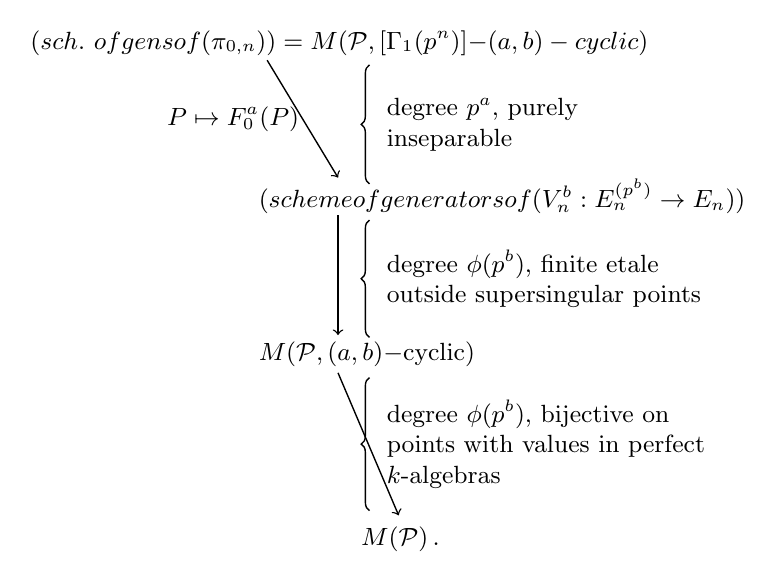
\begin{tikzpicture}[line width=0.5pt, every node/.style={inner sep=1pt, font=\small}]
  \node[anchor=west] (A) at (0,0) {$(\text{sch.\ of gens of } \Ker(\pi_{0,n})) = \mathfrak{M}(\mathcal{P},[\Gamma_1(p^n)]\text{-(a,b)-cyclic})$};
  \node[anchor=west] (B) at (2.9,-1.95) {$(\text{scheme of generators of } \Ker(V_n^b:E_n^{(p^b)}\to E_n))$};
  \node[anchor=west] (C) at (2.9,-3.95) {$\mathfrak{M}(\mathcal{P},(a,b)\text{-\rm cyclic})$};
  \node[anchor=west] (D) at (4.2,-6.3) {$\mathfrak{M}(\mathcal{P})\,.$};
  \draw[->] (3.05,-0.22) -- (3.95,-1.71) node[pos=0.5,left,font=\small] {$P\mapsto F_0^a(P)$};
  \draw[->] (3.95,-2.19) -- (3.95,-3.71);
  \draw[->] (3.95,-4.19) -- (4.72,-6.00);
  \draw[decorate,decoration={brace,amplitude=3pt,mirror}] (4.35,-0.28) -- (4.35,-1.79)
        node[midway,anchor=west,font=\small,align=left,xshift=5pt] {degree $p^a$, purely\\inseparable};
  \draw[decorate,decoration={brace,amplitude=3pt,mirror}] (4.35,-2.25) -- (4.35,-3.74)
        node[midway,anchor=west,font=\small,align=left,xshift=5pt] {degree $\phi(p^b)$, finite etale\\outside supersingular points};
  \draw[decorate,decoration={brace,amplitude=3pt,mirror}] (4.35,-4.25) -- (4.35,-5.94)
        node[midway,anchor=west,font=\small,align=left,xshift=5pt] {degree $\phi(p^b)$, bijective on\\points with values in perfect\\$k$-algebras};
\end{tikzpicture}
\]
\end{kcor}

\begin{proof}
This is just a modular spelling out of the previous corollary.
\end{proof}

\begin{kthm}\label{thm:13.5.4}
Let $k$ be a perfect field of characteristic $p$, $\mathcal{P}$ a representable problem which is finite etale over $(\mathrm{Ell}/k)$. Then the moduli scheme $\mathfrak{M}(\mathcal{P}, [\Gamma_1(p^n)] \tens{\mathbb{Z}} k)$ is the disjoint union, with crossings at the supersingular points, of the $n+1$ $\mathfrak{M}(\mathcal{P})$-schemes
\[
\mathfrak{M}(\mathcal{P}, [\Gamma_1(p^n)]\text{-\rm (a,b) cyclic}) , \quad \text{for } a + b = n .
\]
\end{kthm}

\begin{proof}
Apply the crossings theorem (\ref{thm:13.1.3}).
\end{proof}

\stepcounter{kmitem}
\kmitem\label{item:13.5.6}\emph{Summarizing table}\par
In the table below, $\mathcal{P}$ is a representable problem on $(\mathrm{Ell}/k)$, finite etale over $(\mathrm{Ell}/k)$, with $k$ a perfect field. For both $[\Gamma_0(p^n)]$ and $[\Gamma_1(p^n)]$, we have found expressions for the corresponding $\mathcal{P}$-rigidified modular schemes as disjoint unions of $n+1$ curves (indexed by $(a,b)$ with $a + b = n$) with crossings at the supersingular points. The \emph{multiplicities} given are most easily calculated locally etale on $\mathfrak{M}(\mathcal{P})^{\mathrm{ord}}$, and the formulas in the table may be checked against the computations of the section which follows.

\begin{center}
{\scriptsize
\renewcommand{\arraystretch}{1.35}
\setlength{\tabcolsep}{3pt}
\noindent\textsc{Short Table:} $\Gamma_0(p^n)$ and $\Gamma_1(p^n)$ in char $p$
\par\smallskip
\begin{tabular}{@{}>{\raggedright\arraybackslash}p{3.35cm}|>{\centering\arraybackslash}p{2.45cm}|>{\centering\arraybackslash}p{3.05cm}|}
\hline
& $\mathfrak{M}(\mathcal{P}, [\Gamma_0(p^n)] \tens{\mathbb{Z}} k)$ & $\mathfrak{M}(\mathcal{P}, [\Gamma_1(p^n)] \tens{\mathbb{Z}} k)$ \\
\hline
$(n,0)$-component & & \\
\hline
degree over $\mathfrak{M}(\mathcal{P})$ & $1$ & $\phi(p^n)$ \\
\hline
multiplicity as abstract curve & $1$ & $\phi(p^n)$ \\
\hline
underlying abstract reduced curve, and its degree over $\mathfrak{M}(\mathcal{P})$ & $\mathfrak{M}(\mathcal{P})$; $1$ & $\mathfrak{M}(\mathcal{P})$; $1$ \\
\hline
$(0,n)$-component & & \\
\hline
degree over $\mathfrak{M}(\mathcal{P})$ & $p^n$ & $p^n \phi(p^n)$ \\
\hline
multiplicity as abstract curve & $1$ & $1$ \\
\hline
underlying abstract reduced curve, and its degree over $\mathfrak{M}(\mathcal{P})$ & $\mathfrak{M}(\mathcal{P})^{(\sigma^n)}$ via $(E_n, \beta_n)$, degree $p^n$ & $\mathfrak{M}(\mathcal{P}, [\mathrm{ExIg}(p^n, n)])$, degree $p^n \phi(p^n)$ \\
\hline
$(a,b)$-component with $a, b$ both $\ge 1$ & & \\
\hline
degree over $\mathfrak{M}(\mathcal{P})$ & $\phi(p^b)$ & $\phi(p^n) \phi(p^b)$ \\
\hline
multiplicity as abstract curve & $\phi(p^{\min(a,b)})$ & $\phi(p^a)$ \\
\hline
underlying abstract reduced curve, and its degree over $\mathfrak{M}(\mathcal{P})$ & if $a \ge b$, $\mathfrak{M}(\mathcal{P})$, degree $1$; if $a \le b$, $\mathfrak{M}(\mathcal{P})^{(\sigma^{a-b})}$, degree $p^{b-a}$ & $\mathfrak{M}(\mathcal{P}, [\mathrm{ExIg}(p^b, b)])$, degree $p^b \phi(p^b)$ \\
\hline
\end{tabular}}
\end{center}

\section[Explicit calculations via the groups {$\mathbf{T}[p^n]$} of {$[\Gamma_0(p^n)]$}, {$[\Gamma_1(p^n)]$}]{Explicit calculations via the groups $\mathbf{T}[p^n]$ of \texorpdfstring{$[\Gamma_0(p^n)]$}{[Gamma_0(p^n)]}, \texorpdfstring{$[\Gamma_1(p^n)]$}{[Gamma_1(p^n)]}}
\label{sec:13.6}

\kmitem\label{item:13.6.1}In the previous section we gave a calculation of the moduli scheme $\mathfrak{M}(\mathcal{P},[\Gamma_0(p^n)])$ and $\mathfrak{M}(\mathcal{P},[\Gamma_1(p^n)])$ as $\mathfrak{M}(\mathcal{P})$-schemes, with particular attention to their behavior at the supersingular points. In this section we will analyse what these $\mathfrak{M}(\mathcal{P})$ schemes look like locally (etale) on $\mathfrak{M}(\mathcal{P})^{\mathrm{ord}}$. We have already seen that the covering
\[
\begin{tikzcd}[row sep=1.8em]
\mathfrak{M}(\mathcal{P},[\mathrm{Ig}(p^n)])^{\mathrm{ord}} \arrow[d] \\
\mathfrak{M}(\mathcal{P})^{\mathrm{ord}}
\end{tikzcd}
\]
is a finite etale $(\mathbb{Z}/p^n\mathbb{Z})^\times$-torsor (cf.~\ref{thm:12.6.1}). Over this covering, the universal $E$ has $E[p^n]$ sitting in a short exact sequence
\[
0 \to \mu_{p^n} \to E[p^n] \to \mathbb{Z}/p^n\mathbb{Z} \to 0
\]
for which the $e_{p^n}$-pairing is equal to the unique strongly alternating pairing making $\mu_{p^n}$ and $\mathbb{Z}/p^n\mathbb{Z}$ Cartier dual in the standard way (cf.~\ref{prop:8.10.6}). Therefore Zariski locally on $\mathfrak{M}(\mathcal{P},[\mathrm{Ig}(p^n)])^{\mathrm{ord}}$, there exists a unit $q \in \mathbb{G}_m(\mathfrak{M}(\mathcal{P},[\mathrm{Ig}(p^n)])^{\mathrm{ord}})$ such that $E[p^n]$, in its exact sequence above, is pulled back via $q$ from the group $\mathbf{T}[p^n]$ over $\mathbb{G}_m = \Spec(\mathbb{Z}[q,q^{-1}])$, sitting in its exact sequence
\[
0 \to \mu_{p^n} \to \mathbf{T}[p^n] \to \mathbb{Z}/p^n\mathbb{Z} \to 0 .
\]
In fact, it is a simple matter to compute the $\mathbb{Z}[q,q^{-1}]$-schemes
\[
[\Gamma_0(p^n)]_{\mathbf{T}[p^n]/\mathbb{Z}[q,q^{-1}]}, \qquad [\Gamma_1(p^n)]_{\mathbf{T}[p^n]/\mathbb{Z}[q,q^{-1}]} .
\]

\begin{kprop}\label{prop:13.6.2}
Let $S$ be a connected $\mathbb{Z}[q,q^{-1}]$-scheme, $G \subset \mathbf{T}[p^n] \otimes S$ a finite locally free subgroup of rank $p^n$. Then there exist unique integers $a, b$ both $\ge 0$, $a + b = n$, such that
\[
G \cap \mu_{p^n} = \mu_{p^a}
\]
\[
G \text{ mod } \mu_{p^a} \xrightarrow{\ \sim\ } \mathbb{Z}/p^b\mathbb{Z}
\]
and we have a commutative diagram of short exact sequences of $S$-group-schemes
\[
\begin{tikzcd}[row sep=1.7em, column sep=2.0em]
0 \arrow[r] & \mu_{p^a} \arrow[r] \arrow[d, hook] & G \arrow[r] \arrow[d, hook] & (1/p^b)\mathbb{Z}/\mathbb{Z} \arrow[r] \arrow[d, hook] & 0 \\
0 \arrow[r] & \mu_{p^n} \arrow[r] & \mathbf{T}[p^n] \arrow[r] & (1/p^n)\mathbb{Z}/\mathbb{Z} \arrow[r] & 0 .
\end{tikzcd}
\]
\end{kprop}

\begin{proof}
Simply apply (\ref{cor:4.10.1}) to the composite map
\[
\begin{tikzcd}[row sep=2.3em, column sep=2.8em]
G \arrow[d] \arrow[rd, dashed] & \\
\mathbf{T}[p^n] \arrow[r] & (1/p^n)\mathbb{Z}/\mathbb{Z} ,
\end{tikzcd}
\]
exactly as in the proof of (\ref{prop:13.3.2}).
\end{proof}

\begin{kprop}\label{prop:13.6.3}
Let $S$ be a $\mathbb{Z}[q,q^{-1}]$-scheme, $G \subset \mathbf{T}[p^n] \otimes S$ a finite locally free subgroup of rank $p^n$ and type $(a,b)$ in the sense of the preceding proposition. Let $P \in G(S)$ be a point whose image in $(1/p^n)\mathbb{Z}/\mathbb{Z}$ is $1/p^b$. Then
\begin{enumerate}[label=(\arabic*), leftmargin=2.4em]
\item $G$ is cyclic, with generator $P$, if and only if $p^b P \in \mu_{p^a}(S)$ is a primitive $p^a$'th root of unity.
\item if $Q$ is any point in $\mathbf{T}[p^n](S)$ which projects onto $\lambda/p^b$ in $(1/p^n)\mathbb{Z}/\mathbb{Z}$, for some $\lambda \in (\mathbb{Z}/p^b\mathbb{Z})^\times$, then $Q$ has ``exact order $p^n$'' if and only if $p^b Q \in \mu_{p^n}(S)$ is a primitive $p^a$'th root of unity.
\end{enumerate}
\end{kprop}

\begin{proof}
First we recall that $\mathbf{T}[p^n]$ is embedded as a closed subgroup-scheme of $\mathbb{G}_m \times (1/p^n)\mathbb{Z}/\mathbb{Z}$ for its group-structure (\ref{eq:8.7.2.3}), so by (\ref{prop:1.10.6}) it makes intrinsic sense to speak of a point $Q$ as having ``exact order $p^n$'', and to speak of the cyclic group of rank $p^n$ that $Q$ generates. We have seen that after a faithfully flat extension, $\mathbf{T}[p^n]$ is isomorphic to the kernel of multiplication by $p^n$ in an elliptic curve. This allows us to apply the detailed theory of cyclicity developed in Chapter 6 to $\mathbf{T}[p^n]$.

If $b = 0$, there is nothing to prove for (1). $G$ is the subgroup $\mu_{p^n}$. For (2), if $Q \in \mu_{p^n}(S)$ has ``exact order $p^n$'' in $\mathbf{T}[N]$, then the cyclic $p^n$-group it generates lies entirely inside $\mathbb{G}_m \times \{0\}$ [viewing it as a Cartier divisor inside $\mathbb{G}_m \times ((1/p^n)\mathbb{Z}/\mathbb{Z})$]. Therefore it lies inside $\mu_{p^n} = \mathbf{T}[p^n] \cap (\mathbb{G}_m \times \{0\})$, so must be $\mu_{p^n}$. Therefore $Q$ is necessarily a primitive $p^n$'th root of unity, if it lies in $\mu_{p^n}(S)$ and has ``exact order $p^n$'' in $\mathbf{T}[p^n]$.

If $a = 0$, then $G$ is the $\mathbb{Z}/p^n\mathbb{Z}$ generated by $P$, and $Q$ generates a $\mathbb{Z}/p^n\mathbb{Z}$.

If both $a, b \ge 1$, then (1) and (2) follow from the standard order criterion (\ref{thm:6.7.13}), which automatically applies by (\ref{prop:6.7.8}).
\end{proof}

We now use the explicit form of the group $\mathbf{T}[p^n]$. Let $Q$ be a point in some $\mathbf{T}[p^n](S)$ whose second coordinate is $\lambda/p^b$ for some $\lambda \in (\mathbb{Z}/p^b\mathbb{Z})^\times$ normalized by $0 \le \lambda < p^b$, say
\[
Q = (X, \lambda/p^b)
\]
in the standard coordinates (\ref{eq:8.7.1.2}). Then
\[
p^b Q = (X^{p^b}, \lambda) \sim (X^{p^b}/q^\lambda, 0)
\]
and the requirement is that
\[
X^{p^b}/q^\lambda
\]
be a primitive $p^a$'th root of unity, where $a + b = n$.

In terms of the cyclotomic polynomials, this is the condition
\[
\Phi_{p^a}(X^{p^b}/q^\lambda) = 0 .
\]
Thus we find

\begin{kthm}\label{thm:13.6.4}
For any $n \ge 1$, and any connected $\mathbb{Z}[q,q^{-1}]$-algebra $B$, we have a canonical isomorphism of $B$-schemes
\[
[\Gamma_1(p^n)]_{\mathbf{T}[p^n]/B} \cong \coprod_{\substack{0 \le b \le n \\ a + b = n}} \coprod_{\substack{0 < \lambda < p^b \\ (\lambda, p) = 1}} \Spec\!\left(B[X]/\Phi_{p^a}(X^{p^b}/q^\lambda)\right)
\]
\end{kthm}

\kmitem\label{item:13.6.5}Consider now a cyclic $p^n$-subgroup $G$ of $\mathbf{T}[N]$ over some connected $\mathbb{Z}[q,q^{-1}]$ scheme $S$, which is of type $(a,b)$. If $a = n$, our group $G$ is $\mu_{p^n}$. If $a = 0$, then $b = n$ and our group contains a \emph{unique} element of the form
\[
(X, 1/p^n) .
\]
This element generates it.

If both $a, b \ge 1$, then after passing to a finite locally free covering $S'$ of $S$, $G$ admits a generator of the form
\[
(X, 1/p^b) .
\]
The exact sequence
\[
0 \to \mu_{p^a} \to G \to \left(\frac{1}{p^b}\right)\mathbb{Z}/\mathbb{Z} \to 0
\]
shows that the $X$ above is unique up to multiplication by an element of $\mu_{p^a}$. Therefore by f.p.p.f. descent we have
\[
X^{p^a} \in \Gamma(S, \cO_S) .
\]
We will now see that we can write the equation for $G$ using $X^{p^a}$.

Consider any connected $S$-scheme $S''$, and any element
\[
(Y, \lambda/p^b) \in G(S''), \quad 0 \le \lambda < p^b .
\]
The ``difference''
\[
(Y, \lambda/p^b) - \lambda(X, 1/p^b) = (Y/X^\lambda, 0)
\]
lies in $G$ and has second coordinate zero, so it must lie in $\mu_{p^a}$. Conversely, $\mu_{p^a} \subset G$, and $\lambda(X, 1/p^b) \in G(S)$, so we conclude that
\[
G(S'') = \{(Y, \lambda/p^b) \text{ with } Y^{p^a} = (X^{p^a})^\lambda\} .
\]
Recall that $X$ itself is required to satisfy
\[
\Phi_{p^a}(X^{p^b}/q) = 0
\]
if the point $(X, 1/p^b)$ is to have ``exact order $p^n$.'' For $a \ge 1$, $b \ge 1$, we may write this
\[
0 = \Phi_{p^a}(X^{p^b}/q) = \Phi_p(X^{p^{a+b-1}}/q^{p^{a-1}}) = \Phi_p((X^{p^a})^{p^{b-1}}/q^{p^{a-1}}) .
\]
If we call the quantity $X^{p^a}$ ``$Z$'', then we have a bijective correspondence over any $\mathbb{Z}[q,q^{-1}]$-scheme $S$,
\[
\begin{array}{c}
\left(
\begin{array}{c}
p^n \text{ cyclic subgroups } G \\
\text{of } \mathbf{T}[p^n] \text{ of type } (a,b) \\
\text{with } a, b \text{ both } \ge 1
\end{array}\right)
\longleftrightarrow
\left(
\begin{array}{c}
\text{elements } Z \in \Gamma(S, \cO_S) \\
\text{with} \\
\Phi_p(Z^{p^{b-1}}/q^{p^{a-1}}) = 0
\end{array}\right) \\[6pt]
G_Z \longleftrightarrow Z
\end{array}
\]
where for any connected $S$-scheme $S''$,
\[
G_Z(S'') = \left\{\, (Y, \lambda/p^b) \text{ with } \substack{0 \le \lambda < p^b, \ Y \in \mathbb{G}_m(S'') \\ \text{and } Y^{p^a} = Z^\lambda} \,\right\} .
\]
Putting this all together, we find

\begin{kthm}\label{thm:13.6.6}
For any $n \ge 1$, and any connected $\mathbb{Z}[q,q^{-1}]$-algebra $B$ we have a canonical isomorphism of $B$-schemes
\[
\resizebox{\linewidth}{!}{$\displaystyle
\begin{gathered}
[\Gamma_0(p^n)]_{\mathbf{T}[p^n]/B} \cong \Spec(B) \coprod \Spec(B[X]/(X^{p^n} - q)) \coprod \\[5pt]
\coprod_{\substack{a+b=n \\ a,\, b\text{ both} \ge 1}} \left(\Spec(B[Z]/\Phi_p(Z^{p^{b-1}}/q^{p^{a-1}}))\right) .
\end{gathered}$}
\]
\end{kthm}

If $B$ is an $\mathbb{F}_p[q,q^{-1}]$-algebra, these expressions ``simplify,'' because in $\mathbb{F}_p[X]$ we have, for all $a \ge 1$, the identity
\[
\Phi_{p^a}(X) = (X-1)^{\phi(p^a)} .
\]

\begin{kthm}\label{thm:13.6.7}
If $B$ is any connected $\mathbb{F}_p[q,q^{-1}]$-algebra, we have canonical isomorphisms of $B$-schemes for any $n \ge 1$
\[
\resizebox{\linewidth}{!}{$\displaystyle
\begin{gathered}
[\Gamma_1(p^n)]_{\mathbf{T}[p^n]/B} = \left\{ \coprod_{\substack{0 \le b \le n-1 \\ a+b=n}} \coprod_{\substack{0 < \lambda < p^b \\ (\lambda,p)=1}} \Spec\!\left(B[X]/(X^{p^b}-q^\lambda)^{\phi(p^a)}\right) \right\} \coprod \\[5pt]
\left( \coprod_{\substack{\text{the term} \\ b = n}} \coprod_{\substack{0 < \lambda < p^n \\ (\lambda,p)=1}} \Spec\!\left(B[X]/(X^{p^n}-q^\lambda)\right) \right)
\end{gathered}$}
\]
\[
\resizebox{\linewidth}{!}{$\displaystyle
\begin{gathered}
[\Gamma_0(p^n)]_{\mathbf{T}[p^n]/B} = \{ \Spec(B) \coprod \Spec(B[X]/(X^{p^n}-q)) \coprod \\[5pt]
\left( \coprod_{\substack{a+b=n \\ a \ge 1,\, b \ge 1}} \Spec\!\left(B[Z]/(Z^{p^{b-1}}-q^{p^{a-1}})^{p-1}\right) \right) \} .
\end{gathered}$}
\]
\end{kthm}

\section[The reduction mod {$p$} of {$[\Gamma(p^n)]^{\mathrm{can}}$}]{The reduction mod $p$ of \texorpdfstring{$[\Gamma(p^n)]^{\mathrm{can}}$}{[Gamma(p^n)]^can}}
\label{sec:13.7}

\kmitem\label{item:13.7.1}Let $k$ be a field of characteristic $p$. For every integer $n \ge 1$, there is a unique ring homomorphism
\[
\mathbb{Z}[\zeta_{p^n}] \to k
\]
namely
\[
\zeta_{p^n} \mapsto 1 .
\]
Therefore the moduli problem
\[
[\Gamma(p^n)]^{\mathrm{can}} \tens{\mathbb{Z}[\zeta_{p^n}]} k \quad \text{on } (\mathrm{Ell}/k)
\]
is given by
\[
E/S \mapsto \begin{array}{l}
\text{Drinfeld } p^n\text{-bases } (P,Q) \\
\text{of } E/S \text{ with } e_{p^n}(P,Q) = 1 .
\end{array}
\]
We will denote this moduli problem
\[
[\Gamma(p^n); \det = 1] .
\]
Just as in Chapter 10, we will view such a structure on an $E/S$ as a ``$(\mathbb{Z}/p^n\mathbb{Z})^2$-generator'' of $E[p^n]$, of determinant one, written
\[
\phi : (\mathbb{Z}/p^n\mathbb{Z})^2 \to E[p^n] .
\]
Notice that the \emph{entire} group $\GL(2,\mathbb{Z}/p^n\mathbb{Z})$ operates on the right ($\phi \mapsto \phi \circ g$) on the moduli problem
\[
[\Gamma(p^n); \det = 1] .
\]

\begin{kprop}\label{prop:13.7.2}
Let $E/S/\mathbb{F}_p$ be an ordinary elliptic curve over a connected $\mathbb{F}_p$-scheme, $n \ge 1$ an integer, and
\[
\phi : (\mathbb{Z}/p^n\mathbb{Z})^2 \to E[p^n]
\]
a $[\Gamma(p^n)]$-structure on $E/S$. Then
\begin{enumerate}[label=(\arabic*), leftmargin=2.4em]
\item The composite map $\Lambda = F^n \circ \phi$
\[
\begin{tikzcd}[row sep=2.6em, column sep=2.0em]
& & (\mathbb{Z}/p^n\mathbb{Z})^2 \arrow[d, "\phi"] \arrow[rd, dashed, "\Lambda" description] & & \\
0 \arrow[r] & \Ker F^n \arrow[r] & E[p^n] \arrow[r, "F^n"] & \Ker(V^n) \arrow[r] & 0
\end{tikzcd}
\]
is surjective, its kernel is a constant subgroup of $(\mathbb{Z}/p^n\mathbb{Z})^2$ which is cyclic of order $p^n$, and the quotient
\[
\mathrm{Quot}(\Lambda) \xlongequal{\text{dfn}} (\mathbb{Z}/p^n\mathbb{Z})^2/\Ker(\Lambda)
\]
is a cyclic group of order $p^n$.
\item We have a commutative diagram of short exact sequences of $S$-group-schemes
\[
\begin{tikzcd}[row sep=2.9em, column sep=1.9em]
0 \arrow[r] & \Ker(\Lambda) \arrow[r] \arrow[d, "\phi|_{\Ker(\Lambda)}"] & (\mathbb{Z}/p^n\mathbb{Z})^2 \arrow[r] \arrow[d, "\phi"] & \mathrm{Quot}(\Lambda) \arrow[r] \arrow[d, Rightarrow, shorten >=2pt, shorten <=2pt] & 0 \\
0 \arrow[r] & \Ker(F^n) \arrow[r] & E[p^n] \arrow[r] & \Ker(V^n) \arrow[r] & 0
\end{tikzcd}
\]
in which all the vertical arrows are generators.
\item Any choice of a $\mathbb{Z}/p^n\mathbb{Z}$-basis of $\mathrm{Quot}(\Lambda)$ defines an isomorphism $\mathbb{Z}/p^n\mathbb{Z} \xrightarrow{\ \sim\ } \Ker(V^n)$, which allows us to view $\Lambda$ as a surjective hom from $(\mathbb{Z}/p^n\mathbb{Z})^2$ to $\mathbb{Z}/p^n\mathbb{Z}$. The class of $\Lambda$ in the space
\[
(\mathbb{Z}/p^n\mathbb{Z})^\times \backslash \HomSurj((\mathbb{Z}/p^n\mathbb{Z})^2, \mathbb{Z}/p^n\mathbb{Z})
\]
of component labels (\ref{sec:10.6}) for the trivial subgroup $\{1\} \subset \GL(2,\mathbb{Z}/p^n\mathbb{Z})$ is well-defined independent of choice of basis for $\mathrm{Quot}(\Lambda)$. We will refer to this class as the \emph{component-label} of the $[\Gamma(p^n)]$-structure in question.
\item The $[\Gamma(p^n)]$-structure $\phi$ has determinant one, i.e., satisfies
\[
e_{p^n}\!\left(\phi\binom{1}{0}, \phi\binom{0}{1}\right) = 1 ,
\]
if and only if $\phi|_{\Ker(\Lambda)}$ is the zero-homomorphism.
\end{enumerate}
\end{kprop}

\begin{proof}
Assertions (1), (2), and (3) follow immediately from (\ref{prop:1.11.2}), because by hypothesis $E/S$ is ordinary, so $\Ker(V^n)$ is etale over $S$, locally (etale) on $S$ isomorphic to $\mathbb{Z}/p^n\mathbb{Z}$. To prove (4), we argue as follows. Choose a $\mathbb{Z}/p^n\mathbb{Z}$-basis $k_\Lambda$ of $\Ker(\Lambda)$, and extend it to an oriented basis $(k_\Lambda, \ell_\Lambda)$ of $(\mathbb{Z}/p^n\mathbb{Z})^2$. Then $\ell_\Lambda$ projects to a $\mathbb{Z}/p^n\mathbb{Z}$-basis of $\mathrm{Quot}(\Lambda)$, and $\Lambda(\ell_\Lambda)$ defines an isomorphism $\mathbb{Z}/p^n\mathbb{Z} \xrightarrow{\ \sim\ } \Ker(V^n)$. The dual isomorphism
\[
\Ker(F^n) \xrightarrow{\ \sim\ } \mu_{p^n}
\]
is defined by
\[
\zeta \in \Ker F^n \mapsto e_{p^n}(\zeta, \phi(\ell_\Lambda)) .
\]
Now $\phi|_{\Ker(\Lambda)}$ is the zero-homomorphism if and only if $\phi(k_\Lambda)$ is the zero-section of $\Ker F^n$. Using the above isomorphism we have
\[
\phi(k_\Lambda) = 0 \iff e_{p^n}(\phi(k_\Lambda), \phi(\ell_\Lambda)) = 1 \iff \det \phi = 1 .
\]
\end{proof}

\kmitem\label{item:13.7.3}For each element $\Lambda$ in
\[
(\mathbb{Z}/p^n\mathbb{Z})^\times \backslash \HomSurj((\mathbb{Z}/p^n\mathbb{Z})^2, \mathbb{Z}/p^n\mathbb{Z}) ,
\]
the space of component-labels, we now fix a choice of oriented basis $(k_\Lambda, \ell_\Lambda)$ of $(\mathbb{Z}/p^n\mathbb{Z})^2$ such that $k_\Lambda$ is a $\mathbb{Z}/p^n\mathbb{Z}$-basis of $\Ker(\Lambda)$.

\begin{kcor}\label{cor:13.7.4}
Let $E/S/\mathbb{F}_p$ be an ordinary elliptic curve over a connected $\mathbb{F}_p$-scheme, and let $\phi$ be a $[\Gamma(p^n); \det = 1]$-structure on $E/S$, of component-label $\Lambda$. Then
\begin{enumerate}[label=(\arabic*), leftmargin=2.4em]
\item The point $\phi(\ell_\Lambda) \in E(S)$ is an $[\mathrm{ExIg}(p^n,n)]$-structure (\ref{eq:12.10.5.1}) on $E/S$, i.e., $(0, \phi(\ell_\Lambda))$ is a Drinfeld $p^n$-basis on $E/S$.
\item Given a point $P \in E(S)$ such that $(0,P)$ is a Drinfeld $p^n$-basis of $E/S$, the homomorphism of $S$-group-schemes
\[
\begin{array}{rcl}
(\mathbb{Z}/p^n\mathbb{Z})^2 & \to & E[p^n] \\
k_\Lambda & \mapsto & 0 \\
\ell_\Lambda & \mapsto & P
\end{array}
\]
is a $[\Gamma(p^n); \det = 1]$-structure on $E/S$.
\end{enumerate}
\end{kcor}

\begin{proof}
We have $\phi(k_\Lambda) = 0$.
\end{proof}

\begin{kprop}\label{prop:13.7.5}
Let $E/S/\mathbb{F}_p$ be an elliptic curve, $\Lambda \in (\mathbb{Z}/p^n\mathbb{Z})^\times \backslash \HomSurj$ a component-label, and $(0,P)$ a Drinfeld $p^n$-basis of $E/S$. Then the homomorphism of $S$-group-schemes
\[
\begin{array}{rcl}
(\mathbb{Z}/p^n\mathbb{Z})^2 & \to & E[p^n] \\
k_\Lambda & \mapsto & 0 \\
\ell_\Lambda & \mapsto & P
\end{array}
\]
is a Drinfeld $p^n$-structure on $E/S$, and this construction establishes a functorial bijection
\[
\resizebox{\linewidth}{!}{$\displaystyle
\left\{\begin{array}{c}
[\Gamma(p^n)]\text{-structures on } E/S \text{ with} \\
\phi|_{\Ker(\Lambda)} = 0
\end{array}\right\}
\leftrightarrow
\left\{\begin{array}{c}
[\mathrm{ExIg}(p^n,n)]\text{-structures} \\
\text{on } E/S
\end{array}\right\} .$}
\]
\end{kprop}

\begin{proof}
A tautology!
\end{proof}

\begin{kthm}\label{thm:13.7.6}
Let $k$ be a perfect field of characteristic $p$, $\mathcal{P}$ a representable moduli problem on $(\mathrm{Ell}/k)$ which is finite etale over $(\mathrm{Ell}/k)$. Then
\begin{enumerate}[label=(\arabic*), leftmargin=2.4em]
\item The $\mathfrak{M}(\mathcal{P})$-scheme $\mathfrak{M}(\mathcal{P}, [\Gamma(p^n); \det = 1])$ is the disjoint union, with crossings at the supersingular points, of the $\mathfrak{M}(\mathcal{P})$-schemes
\[
\resizebox{\linewidth}{!}{$\displaystyle
\begin{gathered}
\mathfrak{M}(\mathcal{P}, [\Gamma(p^n)\text{ str. with } \phi(\Ker \Lambda) = 0]) \cong \mathfrak{M}(\mathcal{P}, [\mathrm{ExIg}(p^n,n)]) \\[4pt]
\cong \mathfrak{M}(\mathcal{P}^{(\sigma^{-n})}, [\mathrm{Ig}(p^n)]) \text{ via } \mathrm{pr}_n
\end{gathered}$}
\]
indexed by
\[
(\mathbb{Z}/p^n\mathbb{Z})^\times \backslash \HomSurj((\mathbb{Z}/p^n\mathbb{Z})^2, \mathbb{Z}/p^n\mathbb{Z}) .
\]
\item These are all smooth curves over $k$, finite and flat over $\mathfrak{M}(\mathcal{P})$ of degree $p^n\phi(p^n)$. If $\mathfrak{M}(\mathcal{P})$ is connected (resp.\ geometrically connected), so are the curves $\mathfrak{M}(\mathcal{P}, [\mathrm{ExIg}(p^n,n)])$.
\item The compactified moduli scheme $\overline{\mathfrak{M}}(\mathcal{P}, [\Gamma(p^n); \det = 1])$, viewed as an $\overline{\mathfrak{M}}(\mathcal{P})$-scheme, is the disjoint union, with crossings at the supersingular points, of the compactified moduli schemes
\[
\resizebox{\linewidth}{!}{$\displaystyle
\begin{gathered}
\overline{\mathfrak{M}}(\mathcal{P}, [\Gamma(p^n)\text{-str. with } \phi(\ker \Lambda) = 0]) \cong \overline{\mathfrak{M}}(\mathcal{P}, [\mathrm{ExIg}(p^n,n)]) \\[4pt]
\cong \overline{\mathfrak{M}}(\mathcal{P}^{(\sigma^{-n})}, [\mathrm{Ig}(p^n)]) \text{ via } \mathrm{pr}_n
\end{gathered}$}
\]
indexed by
\[
(\mathbb{Z}/p^n\mathbb{Z})^\times \backslash \HomSurj .
\]
\end{enumerate}
\end{kthm}

\begin{proof}
A straightforward application of the crossings theorem (\ref{thm:13.1.3}) gives (1). Assertion (2) has already been proven (\ref{cor:12.6.2}). For (3), we argue as follows. Because the component curves are all smooth over $k$, and finite over $\mathfrak{M}(\mathcal{P})$, which is itself finite over the $j$-line, over the open set of the $j$-line where $\Phi^{\mathrm{s.s.}}$ is invertible, we have $\mathfrak{M}(\mathcal{P}, [\Gamma(p^n); \det = 1])$ as a disjoint union of Igusa curves. Normalizing a neighborhood of infinity in the $j$-line now gives the assertion.
\end{proof}

\section[Complete local ring of {$[\Gamma(p^n)]^{\mathrm{can}}$} at supersingular points]{Complete local ring of \texorpdfstring{$[\Gamma(p^n)]^{\mathrm{can}}$}{[Gamma(p^n)]^can}, $n \ge 1$, at supersingular points; intersection numbers}
\label{sec:13.8}

\kmitem\label{item:13.8.1}We begin by choosing a convenient set of representatives in
\[
\HomSurj((\mathbb{Z}/p^n\mathbb{Z})^2, \mathbb{Z}/p^n\mathbb{Z})
\]
for the elements of
\[
(\mathbb{Z}/p^n\mathbb{Z})^\times \backslash \HomSurj .
\]
We view elements of $\HomSurj$ as primitive vectors $(x,y)$ with $x, y \in \mathbb{Z}/p^n\mathbb{Z}$, and at least one of $x, y$ a unit. Then a set of representatives modulo the action of $(\mathbb{Z}/p^n\mathbb{Z})^\times$ is provided by the vectors
\[
\left\{\begin{array}{l@{\qquad}l}
(1, -a) & a \in \mathbb{Z}/p^n\mathbb{Z} \quad \text{arbitrary} \\[4pt]
(-pb, 1) & b \in \mathbb{Z}/p^{n-1}\mathbb{Z} \quad \text{arbitrary.}
\end{array}\right.
\]

\kmitem\label{item:13.8.2}With the notations and hypotheses of the previous theorem (\ref{thm:13.7.6}), let $(E/k, a \in \mathcal{P}(E/k))$ be a supersingular point $y_0$ on $\mathfrak{M}(\mathcal{P})$. In terms of the universal formal deformation $E/k[[T]]$ of $E/k$ (to artin local $k$-algebras with residue field $k$), we know that the complete local ring of $\mathfrak{M}(\mathcal{P})$ at $y_0$ is $k[[T]]$. Choose a parameter $X$ for the formal group of $E/k[[T]]$. Then the complete local ring of $\mathfrak{M}(\mathcal{P}, [\Gamma(p^n); \det = 1])$ at the unique point lying over $y_0$ is of the form
\[
k[[x,y]]/(\text{one equation } f)
\]
where $x = X(P)$ and $y = X(Q)$ are the $X$-coordinates of the points $(P,Q)$ of the universal Drinfeld $p^n$-basis of $\det = 1$, (cf.\ the proof of (\ref{thm:13.2.2}), and (\ref{sec:5.4})).

\kmitem\label{item:13.8.3}The condition on the Drinfeld $p^n$-basis $(P,Q)$ that the corresponding $\phi$ satisfy $\phi(\Ker \Lambda) = 0$ is visibly
\begin{equation}\label{eq:13.8.3.1}
\left\{\begin{array}{l@{\quad}l}
P = aQ & \text{if } \Lambda \sim (1, -a) \\[4pt]
pbP = Q & \text{if } \Lambda \sim (-pb, 1) .
\end{array}\right.
\end{equation}
Let us denote, for any $a \in \mathbb{Z}_p$, the series
\begin{equation}\label{eq:13.8.3.2}
\begin{aligned}
{}[a](X) &\in k[[T]][[X]] \\
{}[a](X) &= aX + \text{higher terms}
\end{aligned}
\end{equation}
giving ``multiplication by $a$'' on the formal group of $E/k[[T]]$. If for each element $a \in \mathbb{Z}/p^n\mathbb{Z}$, and for each $b \in \mathbb{Z}/p^{n-1}\mathbb{Z}$, we choose representatives $\tilde a, \tilde b \in \mathbb{Z}_p$, then we may rewrite the above conditions in terms of $x, y$ as
\begin{equation}\label{eq:13.8.3.3}
\left\{\begin{array}{l@{\quad}l}
x = [\tilde a](y) & \text{if } \Lambda \sim (1, -a) \\[4pt]
y = [p\tilde b](x) & \text{if } \Lambda \sim (-pb, 1) .
\end{array}\right.
\end{equation}

\begin{kthm}\label{thm:13.8.4}
Hypotheses and notations as in (\ref{thm:13.7.6}) and (\ref{item:13.8.2}) above, suppose that $y_0$ is a $k$-rational supersingular point on $\mathfrak{M}(\mathcal{P})$. Choose a ring homomorphism $k[[T]] \to k[[x,y]]$ lifting the given $k[[T]] \to k[[x,y]]/(f)$, so that by extension of scalars the formal group law of $E/k[[T]]$ with respect to the parameter $X$ gives rise to a formal group law over $k[[x,y]]$. In terms of this formal group law over $k[[x,y]]$, the complete local ring of $\mathfrak{M}(\mathcal{P}, [\Gamma(p^n); \det = 1])$, $n \ge 1$, at the unique point lying over $y_0$ is isomorphic to
\[
k[[x,y]]\Big/\left( \prod_{a \in \mathbb{Z}/p^n\mathbb{Z}} (x - [\tilde a](y)) \prod_{b \in \mathbb{Z}/p^{n-1}\mathbb{Z}} (y - [p\tilde b](x)) \right) .
\]
In this complete local ring, the closed subscheme $\mathfrak{M}(\mathcal{P},\allowbreak[\Gamma(p^n)]\allowbreak\text{-str. with }\phi(\Ker \Lambda) = 0])$ (cf.\ \ref{thm:13.7.6}) is defined by the single equation
\[
\left\{\begin{array}{l@{\quad}l}
x = [\tilde a]y & \text{if } \Lambda \sim (1, -a) \\[4pt]
y = [p\tilde b]x & \text{if } \Lambda \sim (-pb, 1) .
\end{array}\right.
\]
In particular, $\mathfrak{M}(\mathcal{P}, [\Gamma(p^n); \det = 1])$ is reduced, even at the supersingular points.
\end{kthm}

\begin{proof}
We know this local ring is of the form
\[
k[[x,y]]/(f) ,
\]
with $f$ a non-zero non-unit, and that for each component-label $\Lambda$, the corresponding closed subscheme has complete local ring
\[
\left\{\begin{array}{l@{\qquad}l}
k[[x,y]]/(f, x - [\tilde a](y)) & \text{if } \Lambda \sim (1, -a) , \\[4pt]
k[[x,y]]/(f, y - [p\tilde b](x)) & \text{if } \Lambda \sim (-pb, 1) .
\end{array}\right.
\]
But the $\Lambda$-components are themselves Igusa curves, and at their supersingular points the respective quantities $y, x$ above are parameters (cf.\ the proof of (\ref{thm:12.6.1})). Therefore in the two cases we have isomorphisms
\[
\left\{\begin{array}{l@{\qquad}l}
k[[x,y]]/(f, x - [\tilde a](y)) \xrightarrow{\ \sim\ } k[[y]] , \\[4pt]
k[[x,y]]/(f, y - [p\tilde b](x)) \xrightarrow{\ \sim\ } k[[x]] .
\end{array}\right.
\]
Therefore the complete local rings of the irreducible components are given by
\[
k[[x,y]]/(x - [\tilde a](y)) \qquad \text{if } \Lambda \sim (1, -a) ,
\]
\[
k[[x,y]]/(y - [p\tilde b](x)) \qquad \text{if } \Lambda \sim (-pb, 1) .
\]
The assertion now follows from the crossings theorem (\ref{thm:13.1.3}).
\end{proof}

\begin{kcor}\label{cor:13.8.5}
Hypotheses and notations as above, suppose further that $\mathcal{P}$ is the reduction mod $p$ of a representable problem $\widetilde{\mathcal{P}}$ on $(\mathrm{Ell}/W(k))$ which is finite etale over $(\mathrm{Ell}/W(k))$. Then we may view each $\Lambda$-component
\[
\mathfrak{M}(\mathcal{P}, [\Gamma(p^n)\text{-str. } \phi \text{ with } \phi(\Ker \Lambda) = 0])
\]
as a smooth curve in the regular surface
\[
\mathfrak{M}(\widetilde{\mathcal{P}}, [\Gamma(p^n)]^{\mathrm{can}}) .
\]
If $\Lambda_1$ and $\Lambda_2$ are two distinct component-labels, then the intersection-number of the $\Lambda_1$ and $\Lambda_2$-components at each supersingular point is given by the integer
\[
\left(\#\left((\mathbb{Z}/p^n\mathbb{Z})^2/\Ker(\Lambda_1)+\Ker(\Lambda_2)\right)\right)^2 .
\]
\end{kcor}

\begin{proof}
By definition, the intersection multiplicity in question is the $k$-dimension of the artinian $k$-algebra
\[
\left\{\begin{array}{l@{\quad}c}
k[[x,y]]/(x - [\tilde a_1](y), x - [\tilde a_2](y)) &
\left\{\begin{array}{l}\text{if } \Lambda_1 \sim (1, -a_1) \\ \text{if } \Lambda_2 \sim (1, -a_2)\end{array}\right. \\[12pt]
k[[x,y]]/(x - [\tilde a](y), y - [p\tilde b](x)) &
\left\{\begin{array}{l}\text{if } \Lambda_1 \sim (1, -a) \\ \text{if } \Lambda_2 \sim (-pb, 1)\end{array}\right. \\[12pt]
k[[x,y]]/(y - [p\tilde b_1](x), y - [p\tilde b_2](x)) &
\left\{\begin{array}{l}\text{if } \Lambda_1 \sim (-pb_1, 1) \\ \text{if } \Lambda_2 \sim (-pb_2, 1) .\end{array}\right.
\end{array}\right.
\]
We are claiming that the lengths are respectively given by
\[
(\#(\mathbb{Z}_p/(p^n, \tilde a_1 - \tilde a_2)))^2 , \ 1 , \ (\#(\mathbb{Z}_p/(p^n, p\tilde b_1 - p\tilde b_2)))^2 .
\]
The third case is a special case of the first, with $x$ and $y$ interchanged.

In the second case, the assertion is obvious, because denoting by $\max$ the maximal ideal $\mathrm{M}$ of $k[[x,y]]$, we have
\[
\left\{\begin{array}{l@{\quad}l}
x - [\tilde a](y) \equiv x & \mathrm{mod}\ \max^2 \\[4pt]
y - [p\tilde b](x) \equiv y & \mathrm{mod}\ \max^2 ,
\end{array}\right.
\]
so that these two quantities generate the maximal ideal.

In the first case we have
\[
k[[x,y]]/(x - [\tilde a_1](y)) \xrightarrow{\ \sim\ } k[[y]] ,
\]
with $k[[y]]$ viewed as the complete local ring at a supersingular point on an Igusa curve. The complete local ring at the underlying point on $\mathfrak{M}(\mathcal{P})$ is identified to $k[[T]]$. The formal group law over $k[[y]]$ with which we are dealing is obtained from that of $E/k[[T]]$ with respect to the parameter $X$ by extension of scalars. The ring whose $k$-dimension we are computing is
\[
k[[y]]/([\tilde a_1](y) - [\tilde a_2](y))
\]
\[
\xrightarrow{\ \sim\ } k[[y]]/([\tilde a_1 - \tilde a_2](y)) .
\]
Now write
\[
\tilde a_1 - \tilde a_2 = (\text{unit}) \times p^\nu , \quad 0 \le \nu \le n-1 .
\]
(We have $\nu \le n-1$ because $\Lambda_1$ and $\Lambda_2$ are \emph{distinct} component labels.) Making the change of variable $y \to [\mathrm{unit}](y)$, we may assume
\[
\tilde a_1 - \tilde a_2 = p^\nu , \quad 0 \le \nu \le n-1 ,
\]
and our ring is
\[
k[[y]]/([p^\nu](y)) .
\]
We claim this has length $p^{2\nu}$. The case $\nu = 0$ is obvious, so we may suppose $1 \le \nu \le n-1$. The series $[p^\nu](X)$ is a power series in $X$ with coefficients in the subring $k[[T]]$ of $k[[y]]$ with zero constant term and Weierstrass degree $p^{2\nu}$. Because the Igusa curve of level $n$ sits over $\mathfrak{M}(\mathcal{P})$ by $\mathrm{pr}_n$, it is fully ramified over each supersingular point of degree $p^n\phi(p^n)$. Therefore we have the two congruences
\[
[p^\nu](X) \equiv (\text{elt of } k^\times) X^{p^{2\nu}} \ \mathrm{mod}\ (X^{1+p^{2\nu}}, TX)
\]
\[
T \equiv 0 \ \mathrm{mod}\ (y^{p^n\phi(p^n)}) .
\]
Because $\nu \le n-1$, $p^n\phi(p^n) > p^{2\nu}$, whence we find
\[
[p^\nu](y) \equiv (\text{elt of } k^\times) y^{p^{2\nu}} \ \mathrm{mod}\ (y^{1+p^{2\nu}}) ,
\]
as required.
\end{proof}

\section[Distribution of the cusps on {$[\Gamma(p^n)]^{\mathrm{can}}$}]{Distribution of the cusps on \texorpdfstring{$[\Gamma(p^n)]^{\mathrm{can}}$}{[Gamma(p^n)]^can}}
\label{sec:13.9}

\kmitem\label{item:13.9.1}Let $N \ge 1$ be an integer prime to $p$, $\Gamma \subset \GL(2,\mathbb{Z}/N\mathbb{Z})$ a subgroup, $A$ the ring $(\mathbb{Z}[\zeta_N])^{\det(\Gamma)}$. Suppose that the moduli problem
\[
\mathcal{P} = ([\Gamma(N)]/\Gamma)^{A\text{-can}} \tens{A} A[1/N] \quad \text{on } (\mathrm{Ell}/A[1/N])
\]
is representable. Then the simultaneous moduli problem
\[
(\mathcal{P}, [\Gamma(p^n)]^{\mathrm{can}}) \quad \text{on } (\mathrm{Ell}/A[1/N, \zeta_{p^n}])
\]
is representable, and we have proven (\ref{thm:10.9.4}) that its compactified moduli scheme
\[
\overline{\mathfrak{M}}(\mathcal{P}, [\Gamma(p^n)]^{\mathrm{can}})
\]
is a two-dimensional regular scheme, proper and smooth over $A[\zeta_{p^n}, 1/N]$ outside the supersingular points in characteristic $p$, and that its scheme of cusps is finite etale over $A[\zeta_{p^n}, 1/N]$.

\kmitem\label{item:13.9.2}The cusps are given as a disjoint union of schemes, indexed by the space
\[
\resizebox{\linewidth}{!}{$\displaystyle
\pm 1 \backslash \HomSurj((\mathbb{Z}/p^n\mathbb{Z})^2, \mathbb{Z}/p^n\mathbb{Z}) \times \HomSurj((\mathbb{Z}/N\mathbb{Z})^2, \mathbb{Z}/N\mathbb{Z})/1 \times \Gamma$}
\]
which has a natural projection onto the space
\[
(\mathbb{Z}/p^n\mathbb{Z})^\times \backslash \HomSurj((\mathbb{Z}/p^n\mathbb{Z})^2, \mathbb{Z}/p^n\mathbb{Z}) ,
\]
which indexes the irreducible components of the fiber of
\[
\begin{tikzcd}[row sep=1.9em]
\overline{\mathfrak{M}}(\mathcal{P}, [\Gamma(p^n)]^{\mathrm{can}}) \arrow[d] \\
\Spec(A[1/N, \zeta_{p^n}])
\end{tikzcd}
\]
over any geometric point of the base with characteristic $p$. Recall that by (\ref{prop:8.6.6}), we know that formation of this $\overline{\mathfrak{M}}$, and of its scheme of cusps, commutes with the extensions of scalars
\[
A[1/N, \zeta_{p^n}] \to \text{an algebraically closed field } k \text{ of characteristic } p .
\]
Therefore the finite etale $k$-scheme
\[
\resizebox{\linewidth}{!}{$\displaystyle
\begin{gathered}
\Cusps(\mathcal{P}, [\Gamma(p^n)]^{\mathrm{can}}) \tens{A[1/N, \zeta_{p^n}]} k \\
\xrightarrow{\ \sim\ } \Cusps(\mathcal{P} \tens{A[1/N]} k, [\Gamma(p^n); \det = 1])
\end{gathered}$}
\]
is simultaneously a disjoint union indexed by
\[
\pm 1 \backslash \HomSurj \times \HomSurj/1 \times \Gamma
\]
(when thought of as coming from characteristic zero), and a disjoint union indexed by
\[
(\mathbb{Z}/p^n\mathbb{Z})^\times \backslash \HomSurj((\mathbb{Z}/p^n\mathbb{Z})^2, \mathbb{Z}/p^n\mathbb{Z})
\]
(partitioning in characteristic $p$, according to which irreducible component the cusp lies on).

\begin{kthm}\label{thm:13.9.3}
Hypotheses and notations as above, the natural projection
\[
\begin{tikzcd}[row sep=3.4em]
\begin{gathered} \pm 1 \backslash \HomSurj((\mathbb{Z}/p^n\mathbb{Z})^2, (\mathbb{Z}/p^n\mathbb{Z})) \\ \times\ \HomSurj((\mathbb{Z}/N\mathbb{Z})^2, \mathbb{Z}/N\mathbb{Z})/1 \times \Gamma \end{gathered} \arrow[d] \\
(\mathbb{Z}/p^n\mathbb{Z})^\times \backslash \HomSurj((\mathbb{Z}/p^n\mathbb{Z})^2, \mathbb{Z}/p^n\mathbb{Z})
\end{tikzcd}
\]
is the map which assigns to a cusp-clump in characteristic zero the name of the irreducible component on which it lies in characteristic $p$.
\end{kthm}

\begin{proof}
This compatibility is clear from the way in which the components are labeled, and the fact that over any $\mathbb{F}_p$-algebra $B$, the canonical exact sequence of $B((q))$-group-schemes
\[
0 \to \mu_{p^n} \to \Tate(q)[p^n] \to \mathbb{Z}/p^n\mathbb{Z} \to 0
\]
is canonically isomorphic to the exact sequence
\[
0 \to \Ker F^n \to \Tate(q)[p^n] \to \Ker V^n \to 0 .
\]
\end{proof}

\section[The reduction mod {$p$} of a general {$p$}-power level moduli problem]{The reduction mod $p$ of a general $p$-power level moduli problem}
\label{sec:13.10}

\kmitem\label{item:13.10.1}In this section we fix an integer $n \ge 1$, and consider an arbitrary subgroup
\[
\Gamma \subset \GL(2, \mathbb{Z}/p^n\mathbb{Z}) .
\]
We denote by $A$ the corresponding subring
\[
A = (\mathbb{Z}[\zeta_{p^n}])^{\det(\Gamma)} \subset \mathbb{Z}[\zeta_{p^n}] .
\]
For any field $k$ of characteristic $p$, there is a unique ring homomorphism $A \to k$ (it sends $\zeta_{p^n} \mapsto 1$).

\begin{kthm}\label{thm:13.10.2}
Let $k$ be a field of characteristic $p$, $\mathcal{P}$ a representable moduli problem on $(\mathrm{Ell}/k)$. Denote by $\mathcal{R}$ the moduli problem on $(\mathrm{Ell}/k)$ defined by
\[
\mathcal{R} = ([\Gamma(p^n)]/\Gamma)^{A\text{-can}} \tens{A} k .
\]
Then we have
\begin{enumerate}[label=(\arabic*), leftmargin=2.4em]
\item There is a natural $\mathfrak{M}(\mathcal{P})$-morphism
\[
\mathfrak{M}(\mathcal{P}, [\Gamma(p^n; \det = 1)]) \to \mathfrak{M}(\mathcal{P}, \mathcal{R})
\]
which is $\Gamma$-equivariant, with $\Gamma$ acting on the right on the moduli problem $[\Gamma(p^n); \det = 1]$ by $\phi \mapsto \phi \circ \gamma$, and $\Gamma$ acting trivially on $\mathfrak{M}(\mathcal{P}, \mathcal{R})$.
\item The induced $\mathfrak{M}(\mathcal{P})$-morphism
\[
\mathfrak{M}(\mathcal{P}, [\Gamma(p^n); \det = 1])/\Gamma \to \mathfrak{M}(\mathcal{P}, \mathcal{R})
\]
is surjective, radicial, and integral.
\end{enumerate}
\end{kthm}

\begin{proof}
There is a natural isomorphism of moduli problems on $(\mathrm{Ell}/A)$
\[
([\Gamma(p^n)]/\Gamma)^{A\text{-can}} \xrightarrow{\ \sim\ } [\Gamma(p^n)]^{A\text{-can}}/\Gamma ,
\]
so by general properties of quotients (\ref{thm:7.1.3}, (3)) we have a $\Gamma$-equivariant morphism of $\mathfrak{M}(\mathcal{P})$-schemes
\[
\mathfrak{M}(\mathcal{P}, [\Gamma(p^n)]^{A\text{-can}} \tens{A} k) \to \mathfrak{M}(\mathcal{P}, \mathcal{R})
\]
such that the induced map
\[
\mathfrak{M}(\mathcal{P}, [\Gamma(p^n)]^{A\text{-can}} \tens{A} k)/\Gamma \to \mathfrak{M}(\mathcal{P}, \mathcal{R})
\]
is radicial, surjective and integral (\ref{prop:A7.2.1}). But the natural morphisms of moduli problems on $(\mathrm{Ell}/k)$
\[
\resizebox{\linewidth}{!}{$\displaystyle
\begin{array}{@{}l@{}}
\left([\Gamma(p^n)]^{\mathbb{Z}[\zeta_{p^n}]\text{-can}}\right) \tens{\mathbb{Z}[\zeta_{p^n}]} k \hookrightarrow [\Gamma(p^n)]^{A\text{-can}} \tens{A} k \hookrightarrow [\Gamma(p^n)] \tens{\mathbb{Z}} k
\end{array}$}
\]
are closed immersions which are radicial and surjective, simply because in any $\mathbb{F}_p$-algebra, the $p^n$'th cyclotomic polynomial is
\[
\Phi_{p^n}(X) = (X^{p^{n-1}}-1)^{p-1} = (X-1)^{\phi(p^n)} ,
\]
so that modulo nilpotents \emph{any} Drinfeld $p^n$-basis on an $E/S/\mathbb{F}_p$ has determinant \emph{one}. Therefore the morphism of $\mathfrak{M}(\mathcal{P})$-schemes
\[
\mathfrak{M}(\mathcal{P}, [\Gamma(p^n); \det = 1]) \hookrightarrow \mathfrak{M}(\mathcal{P}, [\Gamma(p^n)]^{A\text{-can}} \tens{A} k)
\]
is a radicial and surjective closed immersion, which is visibly $\Gamma$-equivariant.
\end{proof}

\begin{kthm}\label{thm:13.10.3}
Let $k$ be a perfect field of characteristic $p$, $\mathcal{P}$ a representable moduli problem on $(\mathrm{Ell}/k)$ which is finite etale over $(\mathrm{Ell}/k)$, and such that $\mathfrak{M}(\mathcal{P})$ is connected. For any subgroup
\[
\Gamma \subset \GL(2, \mathbb{Z}/p^n\mathbb{Z}) ,
\]
acting on the $\overline{\mathfrak{M}}(\mathcal{P})$-scheme
\[
\overline{\mathfrak{M}}(\mathcal{P}, [\Gamma(p^n); \det = 1]) ,
\]
we have the following results:
\begin{enumerate}[label=(\arabic*), leftmargin=2.4em]
\item The quotient $\overline{\mathfrak{M}}(\mathcal{P}, [\Gamma(p^n); \det = 1])/\Gamma$ is reduced, it is smooth over $k$ outside its supersingular points, and its supersingular points, with values in any perfect $k$-algebra, map bijectively to those of $\overline{\mathfrak{M}}(\mathcal{P})$.
\item The irreducible components of $\overline{\mathfrak{M}}(\mathcal{P}, [\Gamma(p^n); \det = 1])/\Gamma$ are connected curves over $k$, smooth outside the supersingular points and geometrically unibranch at the supersingular points. They are indexed by the space
\[
(\mathbb{Z}/p^n\mathbb{Z})^\times \backslash \HomSurj((\mathbb{Z}/p^n\mathbb{Z})^2, \mathbb{Z}/p^n\mathbb{Z})/\Gamma
\]
of component labels for $\Gamma$. Each irreducible component is finite and flat over $\overline{\mathfrak{M}}(\mathcal{P})$, and fully ramified over each supersingular point in the sense that its geometric fiber over each supersingular point is a single point.
\item For each $\Lambda \in \HomSurj$, denote by $\mathrm{Fix}^\times(\Lambda) \subset \GL(2,\mathbb{Z}/p^n\mathbb{Z})$ the fixer of the component-label $(\mathbb{Z}/p^n\mathbb{Z})^\times \Lambda$. In the oriented basis $(k_\Lambda, \ell_\Lambda)$ attached to $\Lambda$, $\mathrm{Fix}^\times(\Lambda)$ is the subgroup of all matrices of the form
\[
\left(\begin{array}{cc} * & * \\ 0 & * \end{array}\right) \subset \GL(2, \mathbb{Z}/p^n\mathbb{Z}) .
\]
This group acts on the moduli problem
\[
[\mathrm{ExIg}(p^n, n)] = \text{Drinfeld } p^n\text{-bases of the form } (0,P)
\]
by
\[
\left(\begin{array}{cc} a & b \\ 0 & d \end{array}\right) : (0,P) \mapsto (0, dP) .
\]
With this action understood, the normalization of the irreducible component of $\overline{\mathfrak{M}}(\mathcal{P}, [\Gamma(p^n); \det = 1])/\Gamma$ indexed by $\Lambda$ is the $\overline{\mathfrak{M}}(\mathcal{P})$-scheme
\[
\overline{\mathfrak{M}}(\mathcal{P}, [\mathrm{ExIg}(p^n, n)])/\Gamma \cap \mathrm{Fix}^\times(\Lambda) .
\]
\item If the group $\pm 1$ acts freely on $Z(\mathcal{P})$ (cf.\ (\ref{prop:10.13.7}--\ref{cor:10.13.9})), then the scheme of cusps $j^{-1}(\infty)^{\mathrm{red}}$ in $\overline{\mathfrak{M}}(\mathcal{P}, [\Gamma(p^n); \det = 1])/\Gamma$ is finite etale over the scheme of cusps in $\overline{\mathfrak{M}}(\mathcal{P})$.
\end{enumerate}
\end{kthm}

\begin{proof}
This is immediate from the description (\ref{thm:13.7.6}) of $\overline{\mathfrak{M}}(\mathcal{P}, [\Gamma(p^n); \det = 1])$ as a disjoint union, with crossings at the supersingular points, of the smooth curves
\[
\overline{\mathfrak{M}}(\mathcal{P}, [\Gamma(p^n)\text{ str. } \phi \text{ with } \phi(\Ker \Lambda) = 0]) \cong \overline{\mathfrak{M}}(\mathcal{P}, [\mathrm{ExIg}(p^n, n)])
\]
indexed by $\Lambda \in (\mathbb{Z}/p^n\mathbb{Z})^\times \backslash \HomSurj$ (cf.\ (\ref{thm:12.7.1}) for the last assertion).
\end{proof}
\begin{kthm}\label{thm:13.10.4}
Let $N \ge 1$ be an integer prime to $p$,
\[
\Gamma_2 \subset \GL(2, \Z/N\Z)
\]
a subgroup, $B$ the ring $(\Z[\zeta_N])^{\det(\Gamma_2)}$. Suppose that the moduli problem
\[
\mathcal{P} = ([\Gamma(N)]/\Gamma_2)^{B\text{-can}} \tens{B} B[1/N] \quad \text{on } (\mathrm{Ell}/B[1/N])
\]
is representable, and that $-1$ operates without fixed points on the space of cusp-labels for $\Gamma_2$. Let
\[
\mathcal{R} = ([\Gamma(p^n)]/\Gamma_1)^{A\text{-can}} \quad \text{on } (\mathrm{Ell}/A) .
\]
Let $k$ be a perfect field of characteristic $p$, $B[1/N] \to k$ a ring homomorphism,
\[
A \tens{\Z} B[1/N] \to k
\]
its unique extension to $A \tens{\Z} B[1/N]$. Then
\begin{enumerate}[label=(\arabic*), leftmargin=2.4em]
\item We have a natural morphism of $\mathfrak{M}(\mathcal{P} \tens{} k)$-schemes
\begin{center}
\resizebox{\linewidth}{!}{%
\begin{tikzpicture}[x=1pt,y=1pt,every node/.style={inner sep=0pt}]
  \node[anchor=west] (BL) at (0,0) {$\mathfrak{M}(\mathcal{P} \tens{B[1/N]} k, \mathcal{R} \tens{A} k)$};
  \node[anchor=east] (BR) at (300,0) {$\mathfrak{M}(\mathcal{P} \tens{B[1/N]} k, [\Gamma(p^n); \det = 1])/\Gamma_1$};
  \draw[->] (BR.west) -- (BL.east);
  \node[anchor=south] (TOP) at (150,38) {$\mathfrak{M}(\mathcal{P} \tens{\Z} A, \mathcal{R} \tens{\Z} B[1/N]) \tens{A \tens{\Z} B[1/N]} k$};
  \draw ($(BL.north)+(-9pt,3pt)$) -- ($(BL.north)+(11pt,24pt)$);
  \draw ($(BL.north)+(-6.8pt,2.4pt)$) -- ($(BL.north)+(13.2pt,23.4pt)$);
\end{tikzpicture}}
\end{center}
which is radicial, surjective and integral.
\item If $\Gamma_1$ is balanced (and satisfies $*$ in case $p = 2$ cf.\ \ref{eq:10.10.1.1}), then by (\ref{thm:10.10.3}), the compactified moduli scheme
\[
\overline{\mathfrak{M}}(\mathcal{P} \tens{\Z} A, \mathcal{R} \tens{\Z} B[1/N])
\]
is smooth over $A \tens{} B[1/N]$ outside the supersingular points in characteristic $p$, with scheme of cusps finite etale over $A \tens{} B[1/N]$. There is a natural morphism of $\mathfrak{M}(\mathcal{P} \tens{} k)$-schemes
\begin{center}
\resizebox{\linewidth}{!}{%
\begin{tikzpicture}[x=1pt,y=1pt,every node/.style={inner sep=0pt}]
  \node[anchor=west] (BL) at (0,0) {$\overline{\mathfrak{M}}(\mathcal{P} \tens{B[1/N]} k, \mathcal{R} \tens{A} k)$};
  \node[anchor=east] (BR) at (300,0) {$\overline{\mathfrak{M}}(\mathcal{P} \tens{B[1/N]} k, [\Gamma(p^n); \det = 1])/\Gamma_1$};
  \draw[->] (BR.west) -- (BL.east);
  \node[anchor=south] (TOP) at (150,38) {$\overline{\mathfrak{M}}(\mathcal{P} \tens{\Z} A, \mathcal{R} \tens{\Z} B[1/N]) \tens{A \tens{\Z} B[1/N]} k$};
  \draw ($(BL.north)+(-9pt,3pt)$) -- ($(BL.north)+(11pt,24pt)$);
  \draw ($(BL.north)+(-6.8pt,2.4pt)$) -- ($(BL.north)+(13.2pt,23.4pt)$);
\end{tikzpicture}}
\end{center}
which is radicial, surjective and integral.
\item If $\Gamma_1$ is balanced (and satisfies $*$ in case $p = 2$), this morphism induces an isomorphism on the respective schemes of cusps. Under this isomorphism, the image of the cusp-clump on $\overline{\mathfrak{M}}(\mathcal{P} \tens{\Z} A, \mathcal{R} \tens{\Z} B[1/N])$ labeled by a given cusp-label in
\[
\resizebox{\linewidth}{!}{$\displaystyle
\pm 1 \big\backslash \HomSurj((\Z/p^n\Z)^2, \Z/p^n\Z) \times \HomSurj((\Z/N\Z)^2, \Z/N\Z) \big/ \Gamma_1 \times \Gamma_2$}
\]
lies on the irreducible component labeled by the component-label in
\[
(\Z/p^n\Z)^\times \big\backslash \HomSurj((\Z/p^n\Z)^2, \Z/p^n\Z) \big/ \Gamma_1
\]
\end{enumerate}
\end{kthm}

\begin{proof}
Assertion (1) is just (\ref{thm:13.10.2}). If $\Gamma_1$ is balanced (and satisfies $*$ in case $p = 2$), then the formation of both $\overline{\mathfrak{M}}$ and of its scheme of cusps commutes with the extension of scalars $A \tens{\Z} B[1/N] \to k$. Assertion (2) holds because the compactified schemes in question are the normalizations of $\overline{\mathfrak{M}}(\mathcal{P} \tens{} k)$ in two normal, finite $\overline{\mathfrak{M}}(\mathcal{P} \tens{} k)$-schemes which, over $\mathfrak{M}(\mathcal{P} \tens{} k)$, are given with a radicial surjective $\mathfrak{M}(\mathcal{P} \tens{} k)$-morphism between them. This morphism extends ``by normalization'', and it remains radicial, surjective and integral. Assertion (3) holds because any surjective radicial map between finite etale $k$-schemes (cf.\ (\ref{thm:13.10.3})(4) and (\ref{thm:10.10.3}(6))) is automatically an isomorphism. The labeling compatibility is clear from the construction of the labeling.
\end{proof}

\begin{kcautrem}\label{cautrem:13.10.5}
Even when $\Gamma_1$ is balanced, it is not in general true that the morphisms of \ref{thm:13.10.4}(1) and (3) are isomorphisms outside the supersingular points. For example, if $n \ge 1$ and if $\Gamma_1$ is the entire upper unipotent subgroup
\[
\Gamma_1 = \begin{pmatrix} 1 & * \\ 0 & 1 \end{pmatrix} \subset \GL(2, \Z/p^n\Z) ,
\]
then one easily checks, using (\ref{thm:13.10.3}(3)) and (\ref{cor:5.5.3}), that the source and target of these morphisms have different degrees over $\mathfrak{M}(\mathcal{P} \tens{} k)$ (resp.\ over $\overline{\mathfrak{M}}(\mathcal{P} \tens{} k)$).
\end{kcautrem}

\section[The reduction mod {$p$} of {$\mathrm{[bal.\ \Gamma_1(p^n)]^{\mathrm{can}}}$}]%
{The reduction mod $p$ of \texorpdfstring{$\mathrm{[bal.\ \Gamma_1(p^n)]^{\mathrm{can}}}$}{[bal. Gamma_1(p^n)]\^{}can}}

\kmitem\label{item:13.11.1}
For any field $k$ of characteristic $p$, there is a unique ring homomorphism $\Z[\zeta_{p^n}] \to k$, so the moduli problem
\[
[\mathrm{bal.\ }\Gamma_1(p^n)]^{\mathrm{can}} \tens{\Z[\zeta_{p^n}]} k \quad\text{on } (\Ell/k)
\]
is given by
\begin{equation}\label{eq:13.11.1.1}
\begin{gathered}
E/S \mapsto \text{dual cyclic $p^n$ isogenies } E = E_0 \overset{\pi}{\underset{\pi^t}{\rightleftarrows}} E_n \\
\text{given with } \begin{cases} P_0 \text{ a generator of } \Ker(\pi) \\ Q_n \text{ a generator of } \Ker(\pi^t) , \end{cases} \\
\text{such that under the canonical pairing,} \\
\langle P_0, Q_n \rangle_\pi = 1 .
\end{gathered}
\end{equation}
We will denote this problem
\begin{equation}\label{eq:13.11.1.2}
[\mathrm{bal.\ }\Gamma_1(p^n)\ ;\ \det = 1] .
\end{equation}

\begin{kthm}\label{thm:13.11.2}
Consider a dual pair of cyclic $p^n$ isogenies between ordinary elliptic curves $E_0, E_n$ over a connected $\mathbb{F}_p$-scheme $S$, given with generators of their kernels $P_0, Q_n$, with $\langle P_0, Q_n \rangle = 1$.
\begin{enumerate}[(1)]
\item There exists a unique pair $a,b$ of non-negative integers with $a+b = n$, such that $\pi_{0,n}$ is a cyclic isogeny of type $(a,b)$, and such that $\lambda_{n,0} = (\pi_{0,n})^t$ is a cyclic isogeny of type $(b,a)$.
\item We have $p^b P_0 = 0$, and $(P_0, 0)$ is a Drinfeld $p^b$-basis for $E_0/S$. The point $P_0$ generates a $\Z/p^b\Z$ inside $E_0$, and the quotient of $E_0$ by this subgroup we denote $E_*$. Canonically we have $E_0 \xrightarrow{\ \sim\ } E_*^{(p^b)}$.
\item We have $p^a Q_n = 0$, and $(Q_n, 0)$ is a Drinfeld $p^a$-basis for $E_n/S$. The point $Q_n$ generates a $\Z/p^a\Z$ inside $E_n$, and the quotient of $E_n$ by this subgroup we denote $E_{**}$. Canonically $E_n \xrightarrow{\ \sim\ } E_{**}^{(p^a)}$.
\item There is a unique isomorphism of elliptic curves over $S$
\[
E_* \xrightarrow{\ \sim\ } E_{**}
\]
which makes the upper and lower triangles commute:
\begin{center}
\begin{tikzcd}[column sep=1.8em, row sep=1.8em]
& & E_* \simeq E_{**} \arrow[rrd, "F_{**}^a"] \\
E_*^{(p^b)} \arrow[rru, "V_*^b"] & E_0 \arrow[l, "\sim"'] \arrow[rr, shift left=0.6ex, "\pi_{0,n}"] & & E_n \arrow[ll, shift left=0.6ex, "\lambda_{n,0}"] \arrow[r, "\sim"] & E_{**}^{(p^a)} \arrow[lld, "V_{**}^a"] \\
& & E_* \simeq E_{**} \arrow[llu, "F_*^b"']
\end{tikzcd}
\end{center}
\item In terms of the elliptic curve $E_*$, our original isogeny diagram, in its standard $(a,b)$ factorization, is
\[
E_*^{(p^b)} \overset{F^a}{\underset{V^a}{\rightleftarrows}} E_*^{(p^n)} \overset{V^b}{\underset{F^b}{\rightleftarrows}} E_*^{(p^a)} .
\]
\item The point $P_0 \in E_*^{(p^b)}(S)$ is an $[\mathrm{Ig}(p^b)]$-structure on $E_*/S$, and the point $Q_n \in E_*^{(p^a)}(S)$ is an $[\mathrm{Ig}(p^a)]$-structure on $E_*/S$.
\item If $a \ge b$, there exists a unique unit $u \in (\Z/p^b\Z)^\times$ such that
\[
V_*^{a-b}(Q_n) = u \cdot P_0 \quad\text{in } E_*^{(p^b)}(S) ;
\]
if $b \ge a$, there exists a unique unit $u \in (\Z/p^a\Z)^\times$ such that
\[
Q_n = u \cdot V_*^{b-a}(P_0) \quad\text{in } E_*^{(p^a)}(S) .
\]
\end{enumerate}
\end{kthm}

\begin{proof}
Assertion (1) is just (\ref{thm:13.3.3}). Assertions (2) and (3) are interchanged by duality, so it suffices to prove (2). Consider the standard $(a,b)$ factorization of our cyclic isogeny
\[
P_0\ ;\ E_0 \overset{F_0^a}{\underset{V_0^a}{\rightleftarrows}} E_0^{(p^a)} \simeq E_n^{(p^b)} \overset{V_n^b}{\underset{F_n^b}{\rightleftarrows}} E_n\ ;\ Q_n .
\]
According to (\ref{prop:7.9.2}), $p^b P_0$ generates $\Ker(F_0^a)$, $F_n^b(Q_n)$ generates $\Ker(V_0^a)$, and
\[
\langle p^b P_0, F_n^b(Q_n) \rangle_{F_0^a} = (\langle P_0, Q_n \rangle_{\pi_{0,n}})^{p^b} = (1)^{p^b} = 1 .
\]
But $E_0/S$ being \emph{ordinary}, $F_n^b(Q_n)$ defines an isomorphism
\[
\Z/p^a\Z \xrightarrow{\ \sim\ } \Ker V_0^a ,
\]
and the dual isomorphism
\[
\Ker F_0^a \xrightarrow{\ \sim\ } \mu_{p^a}
\]
is given by
\[
\xi \in \Ker F_0^a \mapsto \langle \xi, F_n^b(Q_n) \rangle_{F_0^a} .
\]
Therefore $p^b P_0$ is the zero-section of $\Ker F_0^a$, because we have
\[
\langle p^b P_0, F_n^b(Q_n) \rangle_{F_0^a} = 1 .
\]
Therefore $p^b P_0 = 0$. Therefore $P_0$ defines a map of $S$-groups
\[
\Z/p^b\Z \to E_0 .
\]
We claim this map is a closed immersion, i.e., that for every geometric point $\Spec(k) \to S$, the image of $P$ in the abstract group $(E_0 \times_S k)(k)$ has exact order $p^b$ in the naive sense. But this is clear, because by (\ref{prop:7.9.2}) the point $F_0^a(P_0) \in E_0^{(p^a)} \simeq E_n^{(p^b)}$ generates $\Ker(V_n^b)$. As $E_n/S$ is \emph{ordinary}, $\Ker(V_n^b)$ is \emph{etale}, so $F_0^a(P_0)$ defines
\[
\Z/p^b\Z \xrightarrow{\ \sim\ } \Ker(V_n^b) .
\]
In particular, $F_0^a(P_0)$ has ``naive exact order $p^b$'' in the group of rational points of every geometric fiber of $E_0^{(p^a)}/S$, and hence $P_0$ has ``naive exact order $p^b$'' in every geometric fiber of $E_0/S$. Therefore $P_0$ does indeed define a closed immersion
\[
\Z/p^b\Z \hookrightarrow E_0/S .
\]
To see that $(P_0, 0)$ is a Drinfeld $p^b$-basis, consider the composite map
\begin{center}
\begin{tikzcd}[column sep=1.8em, row sep=1.8em]
& \Z/p^b\Z \arrow[d] \arrow[rrd, dashed, "F_0^b"] \\
0 \arrow[r] & \Ker F_0^b \arrow[r] & E_0[p^b] \arrow[r] & \Ker V_0^b \arrow[r] & 0 .
\end{tikzcd}
\end{center}
The dotted arrow is certainly injective, because any $\Z/p^b\Z$ inside $E_0[p^b]$ meets $\Ker F_0^b$ only in the zero-section. Comparing ranks, it is an isomorphism, so defines a splitting
\[
E_0[p^b] \simeq \Ker F_0^b \oplus (\text{the } \Z/p^b\Z \text{ generated by } P_0) .
\]
Because zero certainly generates $\Ker F_0^b$, this shows (cf.\ \ref{prop:1.11.2}) that $(0, P_0)$ is a Drinfeld $p^b$-basis of $E_0/S$.

It further shows that the morphism ``multiplication by $p^b$'' on $E_0$ admits a \emph{non-standard factorization}
\begin{center}
\begin{tikzcd}
E_0 \arrow[r] \arrow[rr, bend right=50, "p^b"'] & E_0/(\text{s/gp.\ gen.\ by } P_0) \arrow[r, "F^b"] & E_0 .
\end{tikzcd}
\end{center}
Christening the middle term $E_*$ gives the canonical identification
\[
E_*^{(p^b)} \xrightarrow{\ \sim\ } E_0 .
\]
We now come to the heart of the matter, establishing (4), the isomorphism
\[
E_* \simeq E_{**} .
\]
Once this is done, assertion (5) is obvious by ``substituting'' $E_0 = E_*^{(p^b)}$, $E_n = E_*^{(p^a)}$, and remembering that in the standard $(a,b)$ factorization, the $a$'th term $E_a = E_0^{(p^a)} = E_n^{(p^b)}$. Assertion (6) is ``mise pour memoire'' in view of (2) and (3) (cf.\ \ref{prop:12.2.7}). Assertion (7) holds because the quantities being compared are two generators, over a connected base, of an etale group isomorphic to $\Z/p^{\min(a,b)}\Z$.

To show that $E_* \simeq E_{**}$, we argue as follows. Consider the commutative diagram:
\begin{center}
\begin{tikzcd}[column sep=1.8em, row sep=1.8em]
0 \arrow[r] & \Z/p^a\Z \arrow[r] \arrow[d, "0"] & \Z/p^n\Z \arrow[r] \arrow[d, "P_0"] & \Z/p^b\Z \arrow[r] \arrow[d, "P_0"] & 0 \\
0 \arrow[r] & \Ker(F_0^a) \arrow[r] & \Ker(\pi_{0,n}) \arrow[r, "F_0^a"] & \Ker(\pi_{a,n}) \arrow[r] & 0 .
\end{tikzcd}
\end{center}
The middle vertical arrow is a generator, the term $\Ker(\pi_{a,n})$ is a twisted $\Z/p^b\Z$ (being $\Ker V_n^b$), and $\Ker F_0^a$ is generated by zero. By (\ref{prop:1.11.2}), the final vertical arrow is a generator, hence an isomorphism. Therefore we have a splitting
\[
\Ker(\pi_{0,n}) = \Ker(F_0^a) \oplus (\text{the } \Z/p^b\Z \text{ generated by } P_0) ,
\]
so an \emph{exotic factorization} of
\[
E_0 \xrightarrow{\ \pi_{0,n}\ } E_n
\]
as
\[
E_0 \simeq E_*^{(p^b)} \xrightarrow{\ V_*^b\ } E_* \xrightarrow{\ F_*^a\ } E_*^{(p^a)} .
\]
Therefore we have canonically,
\[
E_n \simeq E_*^{(p^a)} .
\]
Now $E_{**}$ is the \emph{quotient} of $E_n$ by the $\Z/p^a\Z$ generated in it by $Q_n$, while $E_*$ is the quotient of $E_n \simeq E_*^{(p^a)}$ by $\Ker(V_*^a)$. Therefore what we must show is that $Q_n$ in $E_n \simeq E_*^{(p^a)}$ \emph{generates} $\Ker V_*^a$. We know that $Q_n$ generates a $\Z/p^a\Z$ inside $E_n$. So for any connected $S$-scheme $T$, the group generated by $Q_n$ has its only $T$-valued points the multiples of $Q_n$.

So it suffices to show that $Q_n$ lies in $\Ker V_*^a$ (for then the $\Z/p^a\Z$ it generates will lie in $\Ker V_*^a$, and as the ranks are equal the two groups must coincide). To show, finally, that
\[
V_*^a(Q_n) = 0 ,
\]
we resort to a trick.

Because $[\Gamma(p^n)]$ is finite flat over $[\mathrm{bal.\ }\Gamma_1(p^n)]$, it follows (\ref{cor:9.1.9}) that $[\Gamma(p^n)]^{\mathrm{can}}$ is finite flat over $[\mathrm{bal.\ }\Gamma_1(p^n)]^{\mathrm{can}}$. Therefore $[\Gamma(p^n)\ ;\ \det = 1]$ is finite flat over $[\mathrm{bal.\ }\Gamma_1(p^n)\ ;\ \det = 1]$. This means that at the expense of passing to an f.p.p.f.\ $S' \to S$ (certainly allowable for proving $V_*^a(Q_n) = 0$), we may assume given a point $\widetilde{Q} \in E_0(S')$ such that
\[
\begin{cases}
(P_0, \widetilde{Q}) \text{ is a Drinfeld $p^n$-basis on } E_0/S' \text{ with} \\
\qquad e_{p^n}(P_0, \widetilde{Q}) = 1 , \\
\pi_{0,n} \widetilde{Q} = Q_n = \widetilde{Q} \text{ ``}\mathrm{mod}\ P_0\text{.''}
\end{cases}
\]
By our earlier analysis of $[\Gamma(p^n)\ ;\ \det = 1]$-structures on ordinary curves, we know that Zariski locally on $S'$, we have an equation either of the form
\[
\widetilde{Q} = a P_0 , \quad\text{some } a \in \Z/p^n\Z
\]
or of the form
\[
P_0 = p b \widetilde{Q} , \quad\text{some } b \in \Z/p^{n-1}\Z .
\]
In the first case, when $\widetilde{Q}$ lies in the subgroup generated by $P_0$, we have $Q_n = 0$, so certainly $V_*^a(Q_n) = 0$ (in fact $a = 0$ in this case).

In the second case, multiplying $\widetilde{Q}$ and $Q_n$ by a unit in $\Z/p^n\Z$, we may suppose
\[
P_0 = p^\nu \widetilde{Q} \quad\text{for some } \nu \ge 1 .
\]
We claim that $\nu = a$. For if $(p^\nu \widetilde{Q}, \widetilde{Q})$ is a Drinfeld $p^n$-basis, then so is $(0, \widetilde{Q})$, hence, as $E_0/S$ is ordinary, $\widetilde{Q}$ has ``naive exact order $p^n$'' in each geometric fiber of $E_0/S$. Therefore $P_0 = p^\nu \widetilde{Q}$ has ``naive exact order $p^{n-\nu}$'' in each geometric fiber. But $P_0$ has ``naive exact order $p^b$'' in each geometric fiber, so necessarily $\nu = a$.

Now we use the exotic factorization of $\pi_{0,n}$ as
\[
E_*^{(p^b)} \xrightarrow{\ V_*^b\ } E_* \xrightarrow{\ F_*^a\ } E_*^{(p^a)} ,
\]
and compute
\[
\begin{aligned}
V_*^a(Q_n) &= V_*^a(\pi_{0,n}(\widetilde{Q})) \\
&= V_*^a F_*^a V_*^b \widetilde{Q} \\
&= p^a V_*^b \widetilde{Q} \\
&= V_*^b (p^a \widetilde{Q}) \\
&= V_*^b(P_0) .
\end{aligned}
\]
But $V_*^b(P_0) = 0$, because the curve $E_*$ was fabricated exactly so that $E_0 \simeq E_*^{(p^b)}$ with $P_0$ a generator of $\Ker(V_*^b)$!
\end{proof}

\begin{kthm}\label{thm:13.11.3}
Let $a,b$ be integers $\ge 0$, with $a+b = n \ge 1$. Fix a unit
\[
u \in (\Z/p^{\min(a,b)}\Z)^\times .
\]
Let $E/S/\mathbb{F}_p$ be an elliptic curve, given with
\[
\begin{aligned}
P &\in E^{(p^b)}(S) , \text{ a generator of } \Ker(V^b) \\
Q &\in E^{(p^a)}(S) , \text{ a generator of } \Ker(V^a) .
\end{aligned}
\]
Suppose that
\[
\begin{cases}
V^{a-b}(Q) = u P & \text{if } a \ge b \\
Q = u V^{b-a}(P) & \text{if } b \ge a .
\end{cases}
\]
Then:
\begin{enumerate}[(1)]
\item The diagram
\[
P\ ;\ E^{(p^b)} \xrightarrow{\ F^a\ } E^{(p^n)} \xrightarrow{\ V^b\ } E^{(p^a)}\ ;\ Q
\]
is a $[\mathrm{bal.\ }\Gamma_1(p^n)\ ;\ \det = 1]$ structure on $E^{(p^b)}/S$.
\item For any perfect field $k$ of characteristic $p$, and any representable problem $\mathcal{P}$ on $(\Ell/k)$ which is finite etale over $(\Ell/k)$, this construction defines a closed immersion of moduli schemes
\[
\mathfrak{M}(\mathcal{P}, [\mathrm{Ig}(p^{\max(a,b)})]) \hookrightarrow \mathfrak{M}(\mathcal{P}^{(\sigma^b)}, [\mathrm{bal.\ }\Gamma_1(p^n)\ ;\ \det = 1]) .
\]
\end{enumerate}
\end{kthm}

\begin{proof}
We begin with (1). The isogeny
\[
E^{(p^b)} \xrightarrow{\ F^a\ } E^{(p^n)} \xrightarrow{\ V^b\ } E^{(p^a)}
\]
is certainly cyclic in standard order, as follows immediately from the two-step-criterion (\ref{thm:6.7.15}) and the fact that powers of $F$, $V$, and $p$ are all cyclic in characteristic $p$ (cf.\ \ref{lem:12.2.1}--\ref{lem:12.2.5}). That $P \in E^{(p^b)}(S)$ generates the kernel of this composite is clear from the backing-up theorem (\ref{thm:6.7.11}), for as $P$ generates $\Ker(V^b : E^{(p^b)} \to E)$, we certainly have that $F^a(P) = p^a P$ on $(E^{(p^b)})^{(p^a)}$ generates $\Ker(V^b : E^{(p^n)} \to E^{(p^a)})$. Similarly, $Q$ generates the kernel of the dual isogeny. It remains to see that
\[
\langle P, Q \rangle = 1 .
\]
For this we may reduce to the case $u = 1$ simply by replacing $P$ by $\tilde{u} P$ for any $\tilde{u} \in (\Z/p^b\Z)^\times$ which lifts $u$. The question is f.p.p.f.\ local on $S$, so we may suppose there exists a point $R \in E^{(p^n)}(S)$ with
\[
\begin{cases}
V^a(R) = P & \text{if } a \le b \\
V^b(R) = Q & \text{if } a \ge b .
\end{cases}
\]
Then we have
\[
V^a(R) = P \quad\text{and}\quad V^b(R) = Q ,
\]
and since one of $a$ or $b$ is $\ge 1$, $R$ itself must generate $\Ker(V^n)$, by the backing-up criterion (\ref{thm:6.7.11}) applied to $V^n$. Then
\[
\begin{aligned}
\langle P, Q \rangle_{V^b F^a} &= \langle P, V^b(R) \rangle_{V^b F^a} \\
&= \langle V^a(R), V^b(R) \rangle_{V^b F^a} .
\end{aligned}
\]
Again f.p.p.f.\ localizing on $S$, we may assume given a point $R' \in E^{(p^b)}(S)$ with $F^a(R') = R$. Then $p^n R' = 0$, because
\[
\begin{aligned}
p^n R' &= p^b p^a R' = p^b V^a F^a(R') = p^b V^a(R) \\
&= p^b P \\
&= F^b V^b P \\
&= 0 .
\end{aligned}
\]
Therefore
\[
\begin{aligned}
\langle P, Q \rangle_{V^b F^a} &= \langle V^a(R), V^b F^a(R') \rangle_{V^b F^a} \\
&= e_{p^n}(V^a(R), R') \\
&= e_{p^n}(R, F^a(R')) \\
&= e_{p^n}(R, R) = 1 .
\end{aligned}
\]
This proves (1). Therefore the map in (2) is well defined. It is an $\mathfrak{M}(\mathcal{P})$-map between finite $\mathfrak{M}(\mathcal{P})$-schemes, so it is certainly a finite map, so a proper map. So it is a closed immersion if and only if it is an immersion, i.e., injective on $S$-valued points for all $k$-schemes $S$. But this injectivity is clear, for we recover the original object $(E/S, P \text{ and } Q \text{ subject to } u\text{-compatibility})$ from either the source $(E^{(p^b)}\ ;\ P)$ or the target $(E^{(p^a)}\ ;\ Q)$ depending on whether $a \le b$ or $b \le a$, by the inverse of the exotic isomorphism (for $M = \max(a,b)$)
\[
\mathfrak{M}(\mathcal{P}, [\mathrm{Ig}(p^M)]) \xrightarrow{\ \sim\ } \mathfrak{M}(\mathcal{P}^{(\sigma^M)}, [\mathrm{ExIg}(p^M, M)]) .
\]
\end{proof}

\begin{kthm}\label{thm:13.11.4}
Let $k$ be a perfect field of characteristic $p$, $\mathcal{P}$ a representable problem on $(\Ell/k)$ which is finite etale over $(\Ell/k)$. Then
\begin{enumerate}[(1)]
\item the scheme $\mathfrak{M}(\mathcal{P}, [\mathrm{bal.\ }\Gamma_1(p^n)\ ;\ \det = 1])$ is the disjoint union, with crossings at the supersingular points, of the following smooth $k$-curves:
\begin{quote}
for each pair $(a,b)$ of non-negative integers with $a+b = n$, and for each $u \in (\Z/p^{\min(a,b)}\Z)^\times$, one copy of
\[
\mathfrak{M}(\mathcal{P}^{(\sigma^{-b})}, [\mathrm{Ig}(p^{\max(a,b)})]) ,
\]
mapping to $\mathfrak{M}(\mathcal{P})$ by $\mathrm{pr}_b$ (cf.\ \ref{sec:12.10}):
\begin{center}
\begin{tikzcd}
\mathfrak{M}(\mathcal{P}^{(\sigma^{-b})}, [\mathrm{Ig}(p^{\max(a,b)})]) \arrow[d, "\mathrm{pr}_b"] \\
\mathfrak{M}(\mathcal{P})
\end{tikzcd}
\end{center}
\end{quote}
\item the compactified moduli scheme $\overline{\mathfrak{M}}(\mathcal{P}, [\mathrm{bal.\ }\Gamma_1(p^n)\ ;\ \det = 1])$ is the disjoint union, with crossings at the supersingular points, of the following proper smooth $k$-curves:
\begin{quote}
for each $(a,b)$ with $a+b = n$, and for each $u \in (\Z/p^{\min(a,b)}\Z)^\times$, one copy of
\[
\overline{\mathfrak{M}}(\mathcal{P}^{(\sigma^{-b})}, [\mathrm{Ig}(p^{\max(a,b)})]) ,
\]
mapping to $\overline{\mathfrak{M}}(\mathcal{P})$ by $\mathrm{pr}_b$.
\end{quote}
\end{enumerate}
\end{kthm}

\begin{proof}
Statement (1) is just the crossings theorem applied in light of our present analysis, and (2) follows just as in (\ref{thm:13.7.6}).
\end{proof}

\section[The reduction mod {$p$} of quotients of {$\mathrm{[bal.\ \Gamma_1(p^n)]}$} by subgroups of {$\mathrm{(\Z/p^n\Z)^\times \times (\Z/p^n\Z)^\times}$}]%
{The reduction mod $p$ of quotients of \texorpdfstring{$\mathrm{[bal.\ \Gamma_1(p^n)]}$}{[bal. Gamma_1(p^n)]} by subgroups of \texorpdfstring{$(\Z/p^n\Z)^\times \times (\Z/p^n\Z)^\times$}{(Z/p\^{}nZ)\^{}x x (Z/p\^{}nZ)\^{}x}}
\label{sec:13.12}

\kmitem\label{item:13.12.1}
In this section, we fix a subgroup
\[
K \subset (\Z/p^n\Z)^\times \times (\Z/p^n\Z)^\times .
\]
The first and second projections define group-homomorphisms
\begin{equation}\label{eq:13.12.1.1}
\chi_1, \chi_2 : K \to (\Z/p^n\Z)^\times .
\end{equation}
The group $K$ operates on the moduli problem $[\mathrm{bal.\ }\Gamma_1(p^n)]$, by
\begin{equation}\label{eq:13.12.1.2}
\begin{tikzcd}[row sep=1.8em]
P\ ;\ E_0 \rightleftarrows E_n\ ;\ Q \arrow[d, mapsto, "k \in K"] \\
\chi_1(k) P\ ;\ E_0 \rightleftarrows E_n\ ;\ \chi_2(k) Q .
\end{tikzcd}
\end{equation}
If we denote by
\begin{equation}\label{eq:13.12.1.3}
\widetilde{K} \subset \begin{pmatrix} * & * \\ 0 & * \end{pmatrix} \subset \GL(2, \Z/p^n\Z)
\end{equation}
the subgroup consisting of all matrices
\[
\begin{pmatrix} k_1 & * \\ 0 & k_2 \end{pmatrix} \quad (k_1, k_2) \in K,\ * \in \Z/p^n\Z ,
\]
then we have an exact sequence of groups
\begin{equation}\label{eq:13.12.1.4}
0 \to \begin{pmatrix} 1 & * \\ 0 & 1 \end{pmatrix} \to \widetilde{K} \to K \to 0
\end{equation}
whence (\ref{thm:7.4.2}(2)) a canonical isomorphism of moduli problems on $(\Ell/\Z)$
\begin{equation}\label{eq:13.12.1.5}
[\Gamma(p^n)]/\widetilde{K} \simeq [\mathrm{bal.\ }\Gamma_1(p^n)]/K .
\end{equation}

\kmitem\label{item:13.12.2}
Via this identification, we obtain from the general theorem (\ref{thm:13.10.4}) on the reduction mod $p$ of general quotients of $[\Gamma(p^n)]$ by subgroups $\Gamma \subset \GL(2, \Z/p^n\Z)$, a rather concrete theorem on the reduction mod $p$ of quotients of $[\mathrm{bal.\ }\Gamma_1(p^n)]$ by arbitrary subgroups $K$ of $(\Z/p^n\Z)^\times \times (\Z/p^n\Z)^\times$.
\par
In order to state the result concisely, we must introduce some notation. As is customary, we put
\begin{equation}\label{eq:13.12.2.1}
A = (\Z[\zeta_{p^n}])^{\det(K)}
\end{equation}
where by abuse of notation we write
\begin{equation}\label{eq:13.12.2.2}
\det \overset{\mathrm{dfn}}{=} \chi_1\chi_2 : K \to (\Z/p^n\Z)^\times .
\end{equation}
Given a pair of non-negative integers $(a,b)$ with $a+b = n$, we define a subgroup
\[
K(a,b) \subset K
\]
by
\begin{equation}\label{eq:13.12.2.3}
K(a,b) = \{ (k_1, k_2) \in K \text{ with } k_1 \equiv k_2 \bmod p^{\min(a,b)} \} ,
\end{equation}
and a subgroup
\[
\mathrm{Im}\ K(a,b) \subset (\Z/p^{\max(a,b)}\Z)^\times
\]
by
\begin{equation}\label{eq:13.12.2.4}
\mathrm{Im}\ K(a,b) = \begin{cases}
\chi_1(K(a,b)) \bmod p^b & \text{if } a \le b \\
\chi_2(K(a,b)) \bmod p^a & \text{if } a \ge b ,
\end{cases}
\end{equation}
and another subgroup
\[
\mathrm{Comp}\ K(a,b) \subset (\Z/p^{\min(a,b)}\Z)^\times
\]
by
\begin{equation}\label{eq:13.12.2.5}
\mathrm{Comp}\ K(a,b) = (\chi_1/\chi_2)(K) \bmod p^{\min(a,b)} .
\end{equation}
Then we have a short exact sequence
\begin{equation}\label{eq:13.12.2.6}
0 \to K(a,b) \to K \to \mathrm{Comp}\ K(a,b) \to 0
\end{equation}
and a homomorphism
\begin{equation}\label{eq:13.12.2.7}
K(a,b) \twoheadrightarrow \mathrm{Im}\ K(a,b) .
\end{equation}

\begin{kthm}\label{thm:13.12.3}
Let $N \ge 1$ be an integer prime to $p$, $\Gamma \subset \GL(2, \Z/N\Z)$ a subgroup, $B = (\Z[\zeta_N])^{\det(\Gamma)}$ the corresponding ring. Suppose that the moduli problem
\[
\mathcal{P} = ([\Gamma(N)]/\Gamma)^{B\text{-}\mathrm{can}} \tens{B} B[1/N] \quad\text{on } (\Ell/B[1/N])
\]
is representable, and that $-1$ operates without fixed points on the space of cusp labels for $\Gamma$.
\par
Let $K$ be a subgroup of $(\Z/p^n\Z)^\times \times (\Z/p^n\Z)^\times$, and suppose either $p$ odd, or $p^n = 2$, or $\det(K) \equiv 1 \bmod 4$ (so that $K$ satisfies condition $*$). Let $\mathcal{R}$ denote the moduli problem
\[
\mathcal{R} = ([\mathrm{bal.\ }\Gamma_1(p^n)]/K)^{A\text{-}\mathrm{can}} \quad\text{on } (\Ell/A) .
\]
Let $k$ be a perfect field of characteristic $p$, $B[1/N] \to k$ a ring homomorphism, $A \tens{\Z} B[1/N] \to k$ its unique extension to $A \tens{\Z} B[1/N]$. Then
\begin{enumerate}[(1)]
\item We have a radicial, surjective and integral $\overline{\mathfrak{M}}(\mathcal{P} \tens{} k)$-morphism
\begin{center}
\begin{tikzcd}[row sep=1.8em]
\overline{\mathfrak{M}}(\mathcal{P} \tens{} k, [\mathrm{bal.\ }\Gamma_1(p^n)\ ;\ \det = 1])/K \arrow[d] \\
\left( \overline{\mathfrak{M}}(\mathcal{P} \tens{\Z} A, \mathcal{R} \tens{\Z} B[1/N]) \tens{A \tens{\Z} B[1/N]} k \right)^{\mathrm{red}} .
\end{tikzcd}
\end{center}
Source and target are smooth curves over $k$ outside their supersingular points.
\item The irreducible components of the scheme $\overline{\mathfrak{M}}(\mathcal{P} \tens{} k,\allowbreak [\mathrm{bal.\ }\Gamma_1(p^n)\ ;\ \det = 1])/K$ are proper connected curves over $k$, smooth outside the supersingular points and geometrically unibranch at the supersingular points, which are finite flat over $\overline{\mathfrak{M}}(\mathcal{P} \tens{} k)$ and fully ramified (cf.\ \ref{thm:13.10.3}(3)) over each supersingular point. Their normalizations are:
\begin{quote}
for each pair $(a,b)$ of non-negative integers with $a+b = n$, and each element $u$ in $(\Z/p^{\min(a,b)}\Z)^\times /\allowbreak \mathrm{Comp}\ K(a,b)$, one copy of the curve
\[
\overline{\mathfrak{M}}((\mathcal{P} \tens{} k)^{(\sigma^{-b})}, [\mathrm{Ig}(p^{\max(a,b)})])/\mathrm{Im}\ K(a,b)
\]
mapping to $\overline{\mathfrak{M}}(\mathcal{P} \tens{} k)$ by $\mathrm{pr}_b$ (cf.\ \ref{item:12.10.3}).
\end{quote}
\end{enumerate}
\end{kthm}

\begin{proof}
Applying the general theorem (\ref{thm:13.10.4}) to $\mathcal{R}$ viewed as
\[
([\Gamma(p^n)]/\widetilde{K})^{A\text{-}\mathrm{can}} ,
\]
we obtain a radicial, surjective and integral $\overline{\mathfrak{M}}(\mathcal{P} \tens{} k)$-morphism
\begin{center}
\begin{tikzcd}[row sep=1.8em]
\overline{\mathfrak{M}}(\mathcal{P} \tens{} k, [\Gamma(p^n)\ ;\ \det = 1])/\widetilde{K} \arrow[d] \\
\left( \overline{\mathfrak{M}}(\mathcal{P} \tens{\Z} A, \mathcal{R} \tens{\Z} B[1/N]) \tens{A \tens{\Z} B[1/N]} k \right)^{\mathrm{red}} .
\end{tikzcd}
\end{center}
From the exact sequence of groups
\[
0 \to \begin{pmatrix} 1 & * \\ 0 & 1 \end{pmatrix} \to \widetilde{K} \to K \to 0 ,
\]
the source of this morphism may be written
\[
\left( \overline{\mathfrak{M}}(\mathcal{P} \tens{} k, [\Gamma(p^n)\ ;\ \det = 1]) \Big/ \begin{pmatrix} 1 & * \\ 0 & 1 \end{pmatrix} \right) \Big/ K .
\]
We have a natural radicial, surjective and integral map
\[
\resizebox{\linewidth}{!}{$\displaystyle
\overline{\mathfrak{M}}(\mathcal{P} \tens{} k, [\Gamma(p^n)\ ;\ \det = 1]) \Big/ \begin{pmatrix} 1 & * \\ 0 & 1 \end{pmatrix} \longrightarrow \overline{\mathfrak{M}}(\mathcal{P}, [\mathrm{bal.\ }\Gamma_1(p^n)\ ;\ \det = 1])
$}
\]
by (\ref{thm:13.10.4}(2)) applied to the \emph{balanced} subgroup $\begin{pmatrix} 1 & * \\ 0 & 1 \end{pmatrix}$.

This proves (1). Assertion (2) is simply an exercise, in view of the explicit description (\ref{thm:13.11.4}) of the irreducible components of $\overline{\mathfrak{M}}(\mathcal{P} \tens{} k, [\mathrm{bal.\ }\Gamma_1(p^n)\ ;\ \det = 1])$ and of their exact modular description (\ref{thm:13.11.3}) as Igusa curves, which together allow us to ``follow'' the action of $K$ on the set of irreducible components, and to identify the fixer of any $(a,b)$-component as the subgroup $K(a,b)$ of $K$, acting on the corresponding Igusa curve through its quotient $\mathrm{Im}\ K(a,b)$.
\end{proof}

\begin{kcor}\label{cor:13.12.4}
Let $H \subset (\Z/p^n\Z)^\times$ be a subgroup, and suppose that $K$ is the subgroup $H \times H$. If $p = 2$, suppose either $p^n = 2$ or $H \equiv 1 \bmod 4$. Then
\begin{enumerate}[(1)]
\item If $\begin{pmatrix} H & * \\ 0 & H \end{pmatrix}$ is balanced, e.g., if either $n = 1$ and $H$ is arbitrary, or if $n \ge 2$ and $H$ is one of the subgroups $1 + (p^\nu)$ with $\nu \ge [n/2]$, then we have a radicial, surjective and integral morphism
\begin{center}
\begin{tikzcd}[row sep=1.8em]
\overline{\mathfrak{M}}(\mathcal{P} \tens{} k, [\mathrm{bal.\ }\Gamma_1(p^n)\ ;\ \det = 1]) / H \times H \arrow[d] \\
\left( \overline{\mathfrak{M}}(\mathcal{P} \tens{\Z} A, \mathcal{R} \tens{\Z} B[1/N]) \tens{A \tens{\Z} B[1/N]} k \right)^{\mathrm{red}}
\end{tikzcd}
\end{center}
whose source and target are both smooth curves over $k$ outside the supersingular points.
\item The normalizations of the irreducible components of $\overline{\mathfrak{M}}(\mathcal{P} \tens{} k, [\mathrm{bal.\ }\Gamma_1(p^n)\ ;\ \det = 1]) / H \times H$ are the following:
\begin{quote}
for each $(a,b)$ with $a+b = n$, $a,b$ both $\ge 0$, and each $u \in (\Z/p^{\min(a,b)}\Z)^\times / (\text{image of } H \bmod p^{\min(a,b)}) ,$ one copy of
\[
\resizebox{\linewidth}{!}{$\displaystyle
\overline{\mathfrak{M}}((\mathcal{P} \tens{} k)^{(\sigma^{-b})}, [\mathrm{Ig}(p^{\max(a,b)})]) / (\text{image of } H \bmod p^{\max(a,b)}) ,
$}
\]
mapping to $\overline{\mathfrak{M}}(\mathcal{P} \tens{} k)$ by $\mathrm{pr}_b$.
\end{quote}
\item If $n = 1$, and $H$ is an arbitrary subgroup of $\mathbb{F}_p^\times$, then there are exactly \emph{two} irreducible components, indexed by $(1,0)$ and $(0,1)$, whose normalizations are
\begin{itemize}[leftmargin=2.5em]
\item[$(1,0)$~:] $\overline{\mathfrak{M}}(\mathcal{P} \tens{} k, [\mathrm{Ig}(p)])/H$ mapping by usual $\mathrm{pr}$ to $\overline{\mathfrak{M}}(\mathcal{P} \tens{} k)$.
\item[$(0,1)$~:] $\overline{\mathfrak{M}}((\mathcal{P} \tens{} k)^{(\sigma^{-1})}, [\mathrm{Ig}(p)])/H$ mapping by $\mathrm{pr}_1$ to $\overline{\mathfrak{M}}(\mathcal{P} \tens{} k)$.
\end{itemize}
\item If $n \ge 2$, and $H$ is the subgroup $1 + (p^\nu)$ with $\nu \ge [n/2]$, then $H \bmod p^{\min(a,b)}$ is always trivial, so the normalizations of the irreducible components are
\begin{quote}
for each $(a,b)$ with $a+b = n$, $a,b$ both $\ge 0$, and for each $u \in (\Z/p^{\min(a,b)}\Z)^\times$, one copy of
\[
\overline{\mathfrak{M}}((\mathcal{P} \tens{} k)^{(\sigma^{-b})}, [\mathrm{Ig}(p^{\min(\nu, \max(a,b))})])
\]
mapping to $\overline{\mathfrak{M}}(\mathcal{P} \tens{} k)$ by $\mathrm{pr}_b$.
\end{quote}
\end{enumerate}
\end{kcor}

\begin{proof}
Assertion (1) is a special case of (\ref{thm:13.12.3}), in virtue of the theorem (\ref{thm:10.10.3}(6)) on balanced subgroups giving \emph{reduced} special fibers outside the supersingular points. Assertions (2), (3), (4) are just spellings-out of the previous theorem in the particular case $K = H \times H$.
\end{proof}
